%%%%%%%%%%%%%%%%%%%%%%%%%%%%%%%%%%%%%%%%%%%%%%%%%%%%%%%%%%%%%%%%%%%%%%%%%%%%
% AGUJournalTemplate.tex: this template file is for articles formatted with LaTeX
%
% This file includes commands and instructions
% given in the order necessary to produce a final output that will
% satisfy AGU requirements, including customized APA reference formatting.
%
% You may copy this file and give it your
% article name, and enter your text.
%
%
% Step 1: Set the \documentclass
%
%

%% To submit your paper:
\documentclass[draft]{agujournal2019}
\usepackage{url} %this package should fix any errors with URLs in refs.
\usepackage{lineno}
\usepackage[inline]{trackchanges} %for better track changes. finalnew option will compile document with changes incorporated.
\usepackage{soul}
\linenumbers
\usepackage{graphicx}
\usepackage{amsmath,amsfonts,amsthm,bm}
\DeclareMathOperator{\tr}{Tr}
\usepackage{amssymb}
\usepackage[fleqn,tbtags]{mathtools}
\usepackage{tensor}
\usepackage{breakcites}
\usepackage{siunitx}
\usepackage{multirow}
\usepackage{xcolor}
\usepackage[super]{nth}
\usepackage[geometry]{ifsym}
\usepackage{multirow}
%\usepackage[utf8]{inputenc}
%\usepackage{epstopdf}

\renewcommand{\Re}{\operatorname{Re} } 
\renewcommand{\Im}{\operatorname{Im} } 

%%%%%%%
% As of 2018 we recommend use of the TrackChanges package to mark revisions.
% The trackchanges package adds five new LaTeX commands:
%
%  \note[editor]{The note}
%  \annote[editor]{Text to annotate}{The note}
%  \add[editor]{Text to add}
%  \remove[editor]{Text to remove}
%  \change[editor]{Text to remove}{Text to add}
%
% complete documentation is here: http://trackchanges.sourceforge.net/
%%%%%%%

\draftfalse

%% Enter journal name below.
%% Choose from this list of Journals:
%
% JGR: Atmospheres
% JGR: Biogeosciences
% JGR: Earth Surface
% JGR: Oceans
% JGR: Planets
% JGR: Solid Earth
% JGR: Space Physics
% Global Biogeochemical Cycles
% Geophysical Research Letters
% Paleoceanography and Paleoclimatology
% Radio Science
% Reviews of Geophysics
% Tectonics
% Space Weather
% Water Resources Research
% Geochemistry, Geophysics, Geosystems
% Journal of Advances in Modeling Earth Systems (JAMES)
% Earth's Future
% Earth and Space Science
% Geohealth
%
% ie, \journalname{Water Resources Research}
\linespread{2.2}
\journalname{JGR: Solid Earth}


\begin{document}

%------------------------------------------------------------------------ 
%  Title
%------------------------------------------------------------------------ 

\title{Homogenization of porous seismic thin layers with internal stratification for reflectivity applications}
 %------------------------------------------------------------------------ %%
%
%  AUTHORS AND AFFILIATIONS
%
%% %------------------------------------------------------------------------ 

\authors{Edith Sotelo\affil{1}, Nicol\'{a}s D. Barbosa\affil{1}, Santiago G. Solazzi\affil{1}, J. Germ\'{a}n Rubino\affil{2}, Marco Favino\affil{1}, Klaus Holliger\affil{1} }


 \affiliation{1}{Institute of Earth Sciences, University of Lausanne, Lausanne, Switzerland }
 \affiliation{2}{CONICET, Centro Atómico Bariloche - CNEA, San Carlos de Bariloche, Argentina}

\correspondingauthor{Edith Sotelo}{edith.sotelogamboa@unil.ch}

%% Keypoints, final entry on title page.

\begin{keypoints}
\item We propose a procedure to homogenize the seismic properties of porous thin layers composed of a non-periodic sequence of strata.
\item This procedure incorporates the boundary conditions induced by the embedding  background, which is assumed to be impermeable.
\item The resulting viscoelastic equivalents accurately reproduce the seismic P-wave reflectivities of the porous thin layers.

\end{keypoints}

%------------------------------------------------------------------------ %%
%  ABSTRACT and PLAIN LANGUAGE SUMMARY
%% %------------------------------------------------------------------------ 

\begin{abstract}
Stratified thin layers often present a prominent mechanical contrast with regard to the embedding background and, hence, are important targets for seismic reflection studies. An efficient way to study the reflectivity response of these thin layers is to employ their homogenized viscoelastic equivalents.
We aim to homogenize a simple, yet realistic, thin-layer model, which is composed  of a finite non-periodic sequence of homogeneous porous strata embedded in a background deemed impermeable at the seismic frequencies. The overarching objective is to reproduce the reflectivity response of such stratified thin layers.
However, the estimation of the equivalent moduli is inherently affected by the boundary conditions (BC) associated with the embedding background. Therefore, classical homogenization procedures, which assume the existence of a periodic structure, are not readily applicable. We, therefore, propose a novel homogenization procedure that incorporates naturally the appropriate BC. To this end, we consider a sample that includes both a part of the background and a section of the thin layer, to which we apply classical oscillatory relaxation tests. However, we estimate the average of stress and strain components only over the thin layer section of interest. To test the accuracy of the method, we consider a sandstone composed of two strata saturated with different fluids embedded in impermeable half-spaces. After estimating the corresponding equivalent moduli, we compare the resulting P-wave reflectivities with those obtained using the original model. 
Our results show that the inferred viscoelastic equivalent closely reproduces the reflectivities of the stratified thin layer in the seismic frequency range.
\end{abstract}

\section*{Plain Language Summary}
Layer-type geological structures are relevant for a wide range of pertinent  applications such as carbon sequestration or hydrocarbon exploration since they can serve as storage of fluids of interest. The seismic method is commonly employed to detect the interfaces between different layers using the corresponding reflected wave. Layers are considered to be thin from a seismic point of view when they are below the resolution of the employed seismic methods. If a thin layer contains a periodic distribution of interfaces such as a repeating sequence of strata or beds, methods exist to obtain a homogenized version of such structure.
However, in the presence of a finite, non-periodic number of strata, these established methodologies are not applicable. We propose a novel approach to compute homogenized properties of thin layers composed of a non-periodic sequence of strata for seismic reflectivity studies.  


%% ------------------------------------------------------------------------ %%
%
%  TEXT
%
%% ------------------------------------------------------------------------ %%

\section{Introduction}
Quantitative interpretation of seismic reflection data is essential for constraining rock and pore fluid properties in general and for characterizing seismic-scale thin layers in particular. In the given context, a layer is considered to be thin if the seismic reflections from the top and bottom interfaces cannot be individually resolved at the dominant wavelength, such that their compounded effect manifests itself as a single seismic reflection signal. This effect occurs when the layer thickness is equal to or smaller than a quarter of the dominant wavelength \cite{Widess1973, Kallweit1982}.
The corresponding threshold is known as the tuning thickness and is characterized by an initial constructive interference of the reflection signals from the top and bottom interfaces that becomes destructive as the layer thickness decreases \cite{Bakke1998, Hamlyn2014}. Thin layers commonly exhibit heterogeneous structures \cite<e.g.,>{Li2020, Hussain2023}, such as internal stratification (Figure \ref{fig.1}a), which, in turn, govern their effective seismic response.
Pertinent applications of reflectivity studies on thin layers are, for instance,  the characterization of gas-bearing beds \cite<e.g.,>{Cichostepski2019, Shakir2022} 
as well as the monitoring of carbon sequestration \cite<e.g.,>{Williams2012,Zhang2013}. Current methodologies to estimate the rock properties of thin layers have been largely developed within the elastic framework \cite<e.g.,>{Puryear2008,Rubino2009a,Zhang2013, Romdhane2014, Huang2016}. Since the theory of elasticity cannot account for fluid-solid interactions in heterogenoues porous rocks, this approach is likely to affect the accuracy of the estimated properties

Conversely, using  a poroelastic framework allows for an accurate physical description of heterogenous porous rocks in general and thin layers saturated with different fluids, in particular. Evidence suggests that heterogenoues poroelastic media
exhibit equivalent viscoelastic behaviors regarding attenuation and velocity dispersion in the seismic frequency range. \cite<e.g.,>{Pride2004, Carcione2006}. This dispersive behavior is the consequence of an energy dissipation phenomenon known as wave-induced fluid flow or WIFF \cite<e.g.,>{Muller2010} that occurs when a passing seismic wave generates pressure gradients between different parts of a poroelastic medium
that equilibrate by fluid flow.
For typical seismic frequencies, WIFF occurs predominantly in the mesoscopic scale range \cite<e.g.,>{Pride2004, Muller2010}. This refers to  WIFF taking place between  heterogeneities that are much larger than the prevailing pore size  but much smaller than the wavelength \cite<e.g.,>{Norris1993}. In this context, the substitution of a heterogeneous thin layer by the corresponding homogenized viscoelastic representation can be deemed as an efficient technique to study its seismic reflectivity response. Indeed, previous work
demonstrates the applicability of the poroelastic-to-viscoelastic homogenization approach to frequency-dependent seismic reflection studies of thin layers. For instance, \citeA{Rubino2011} and \citeA{Rubino2011a} employ viscoelastic substitutes to represent thin sandstone layers presenting different patchy saturations of CO$_2$ to investigate the corresponding effects on zero-offset seismic reflection data as well as on
the variation of amplitudes for different incidence angles. Similarly,
\citeA{He2020} use viscoelastic substitutes of thin fractured layers to investigate their impact on the P-wave amplitude variation with respect to the incidence angle and frequency. Moreover, \citeA{Jin2017} employ an equivalent viscoelastic representation to replace a partially gas-saturated thin layer. In the same study, this model is later used to estimate gas saturation and layer thickness from seismic amplitude variations with the incidence angle and frequency.

The pioneering work of \citeA{White1975a} and \citeA{White1975} is one of the first to show the equivalent viscoelastic behavior of simple poroelastic composites saturated with gas and water. In particular, their periodic model of alternating  porous beds \cite{White1975} has been used to represent herogeneous thin layers with an internal stratification \cite<e.g.,>{Quintal2009,He2020}. 
In this modeling approach, a porous thin layer is assumed to be embedded in an impermeable background and to consist of a stack of periodically alternating beds that are deemed poroelastic, homogeneous and isotropic. This hydraulically isolated thin-layer model is useful to represent relevant scenarios for subsurface applications such as the case of a thin layer composed by a sand-shale sequence  surrounded by impermeable shale \cite<e.g.,>{Li2020}. Another pertinent scenario scenario corresponds to porous systems consisting of a main fault or fracture surrounded by a thin damage zone, that is embedded in impermeable intact rock \cite<e.g.,>{Caine1996, Mitchell2012}. Several studies have applied the aforementioned model to investigate the frequency-dependent reflectivity response of thin layers of interest.
For instance, \citeauthor{Quintal2009} \citeyear{Quintal2009, Quintal2011a}
%\citeA{Quintal2009} %and \citeA{Quintal2011a}
compare the frequency-dependent reflection coefficients at normal incidence of viscoelastic substitutes of thin-layer models  consisting of a stack of periodically
alternating sandstones with differing rock and fluid properties
embedded in elastic background. Whereas, \citeA{He2020} utilize a particular version of this model to represent a thin layer containing fractures. They assume that the thin layer is embedded in impermeable shale and that one of its alternating beds represents a horizontal fracture with a much higher permeability, softer moduli and smaller thickness than the other bed \cite{Brajanovski2005,Kong2013}. In their study, they use viscoelastic substitutes of these fractured thin layers to examine the effect of various saturating fluids and fracture properties on the variation of seismic amplitude as a function of the angle of incidence and frequency.

A general assumption in the homogenization of a porous medium containing a deterministic heterogeneous structure is its periodicity, for example, an ensemble of beds that repeats a sufficient number of times so that its
equivalent behavior is, for practical purposes, unaffected by the boundary conditions (BC) induced by the surrounding rock \cite<e.g.,>{Wenzlau2010, Quintal2011}. Arguably, a more realistic way to conceptualize a stratified porous thin layer is to consider a model where the thin layer is comprised of a finite non-periodic stratigraphic sequence (Figure \ref{fig.1}a). However, in this case, boundary effects associated with the background embedding the thin layer inherently affect the estimation of the equivalent moduli. Classical homogenization methodologies are not readily applicable to this type of thin-layer models, and the development of alternative suitable procedures remain largely unexplored.

In this work, we seek to alleviate this problem by proposing a method to homogenize non-periodically stratified porous thin layers embedded in a background deemed impermeable for the frequencies of interest. The overarching objective is to use the homogenized medium to predict the seismic reflectivity of the porous thin layer.
To this end, the proposed method, which we describe in the following, incorporates the influence of the BC induced by the embedding background for the estimation of the corresponding equivalent moduli.
We test the accuracy of the proposed method using a thin-layer model that consists of a sequence of two  porous sandstone beds embedded between two impermeable half-spaces. We estimate the corresponding equivalent moduli by applying the proposed homogenization procedure and then calculate P-wave reflectivities at the interface between the upper half-space and the homogenized equivalent representation of the thin layer. Finally, we compare these results against those obtained using the original porous thin layer.
 
\section{Theory and Methods}
In this section, we first detail the theoretical aspects regarding the validity of the poroelastic-to-viscoelastic equivalence. Then, we introduce the proposed homogenization procedure to estimate the equivalent moduli of an infinite horizontal thin layer embedded in half-spaces that are deemed impermeable for the frequencies of interest.  
The evaluation of the reflectivity, using  semi-analytical plane-wave solutions, for the proposed poroelastic thin-layer model and its corresponding viscoelastic equivalent are detailed in Appendices A and B, respectively.

\begin{figure}[!ht]
\centering
        \includegraphics[ width= 120mm, height=70mm]{Figure1.eps}
\caption{ (a) Schematic illustration of a stratified thin-layer model composed of a sequence of four distinct poroelastic beds B1, B2, B3 and B4. This thin layer is embedded in the half-spaces $\Lambda_1$ and $\Lambda_2$ deemed impermeable for the frequencies of interest. The light blue box represents a sample $\Omega_e$ used for the proposed homogenization procedure. (b) Enlarged view of the sample $\Omega_e = \Omega_p \, \cup \, \Omega_b$, where  $\Omega_p$ is a representative section of the thin layer and  $\Omega_b= \Omega_{b1}  \, \cup \, \Omega_{b2}$ is a portion of the background, with $\Omega_{b1} \subset \Lambda_1$ and $\Omega_{b2} \subset \Lambda_2$, respectively. $\Gamma$ is the boundary of the  sample $\Omega_e$, with  $\Gamma = \Gamma_1^+ \cup \Gamma_1^- \cup \Gamma_3^+ \cup \Gamma_3^-$.
}
\label{fig.1}
\end{figure}

\subsection{Mesoscale fluid pressure diffusion}
WIFF occurs when a seismic wave propagating through a heterogeneous poroelastic medium creates
pressure gradients that equilibrate by fluid flow \cite{Muller2010}.
We focus on WIFF prevailing between mesoscale heterogeneities since this is particularly relevant for seismic applications. Mesoscale heterogeneities have a characteristic size $L_m$ that is much larger than the pore size $L_p$ but much smaller than the wavelength $\lambda_w$. For instance, for a thin layer consisting of a sequence of homogeneous porous beds, the size of the mesoscale heterogeneity is dictated by the thickness of these beds.
For sufficiently low frequencies $f$, which are generally within the seismic range, the drag force at the solid-fluid interface associated with WIFF is viscous-dominated \cite{Johnson1987} and, fluid pressure diffusion (FPD) is the mechanism driving WIFF \cite{Pride2005}. The reference frequency that is associated with the transition from viscous- towards inertia-dominated drag forces is Biot's characteristic frequency $f_B$ \cite{Biot1956, Dutta1979}
\begin{linenomath*}
\begin{equation}\label{Eq.1}
f_B= \frac{1}{2 \pi} \frac{\eta \phi}{ \rho_f \kappa S },
\end{equation}
\end{linenomath*}
where $\phi$ is the porosity, $\kappa$  the static permeability, $\eta$, the fluid viscosity,  $\rho_f$ the fluid density, and $S$ the tortuosity of the pore space. The aforementioned considerations regarding scales and frequencies that frame mesoscale WIFF driven by FPD can be thus summarized as
\begin{linenomath*}
\begin{equation}\label{Eq.2}
\begin{split}
 L_p & \ll L_m \ll \lambda_w, \\
f & \ll f_B.
\end{split}
\end{equation}
\end{linenomath*}

It can be shown that the equation governing this FPD mechanism stems from \citeauthor{Biot1941}'s \citeyear{Biot1941} quasi-static equations \cite{Dutta1979, Chandler1981, Norris1993}, where the corresponding diffusion coefficient $D$ together with its characteristic diffusion length $L_d$ can be expressed as \cite{Norris1993}
\begin{linenomath*}
\begin{equation}\label{Eq.3}
\begin{split}
&D= \frac {\kappa} {\eta} \frac{M H_d}{H},\\
&L_d=\sqrt{\frac{D}{\omega}},
\end{split}
\end{equation}
\end{linenomath*}
where $M$ is Biot’s fluid storage modulus, $H_d$ and $H$ are the drained and undrained plane-wave moduli, respectively, and $\omega$ is the angular frequency $\omega = 2 \pi f$.
The required rock physical properties are
\begin{linenomath*}
\begin{equation}\label{Eq.4}
\begin{split}
& H_d = \lambda_d + 2 \mu, \\
& H = H_d + M \alpha ^2, \\
& \lambda_d= K_m - \frac{2}{3} \mu, \\
& \alpha =1-\frac{K_m}{K_s},\\
& M  =\left( \frac{\alpha-\phi}{K_s} +\frac{\phi}{K_f} \right)^{-1},
\end{split}
\end{equation}
\end{linenomath*}
where $\lambda_d$ is the drained Lamé modulus, $\mu$ is the shear modulus, $\alpha$ is the Biot-Willis equivalent stress coefficient, and $K_m$, $K_s$, and $K_f$ are the bulk moduli of the drained solid frame, the solid grains, and the pore fluid, respectively.

The frequency, the characteristic diffusion length $L_d$, and the size of the heterogeneity $L_m$ control the so-called relaxed and unrelaxed FPD regimes \cite{Muller2010}. The relaxed state prevails at sufficiently low frequencies, for which  $L_d \gg L_m$. In this regime, there is enough time for the pressure between the beds to equilibrate. Conversely, the unrelaxed state prevails at sufficiently high frequencies, for which $L_d \ll L_m$. Consequently, there is insufficient time for pressure equilibration to take place and, hence, the different beds behave as hydraulically isolated. A transition zone exists at intermediate frequencies, for which $L_d \approx L_m$.
This zone is associated with attenuation and dispersion of body waves due to viscous dissipation. The maximum dissipation energy is related to a characteristic transition frequency $f_c= \omega_c/2\pi$, which depends on the diffusion coefficient $D$ and the characteristic size of the heterogeneity $L_m$ \cite{Muller2006}
\begin{linenomath*}
\begin{equation}\label{Eq.5}
\omega_c \approx \frac{D}{(L_m)^2}.
\end{equation}
\end{linenomath*}

The described FPD relaxation mechanism produces a viscoelastic behavior of the thin layer under consideration. The frequency-dependent moduli that describe such a viscoelastic material can be estimated by solving \citeauthor{Biot1941}'s \citeyear{Biot1941} quasi-static equations over a representative sample of the thin-layer model (Figure \ref{fig.1}) by performing oscillatory relaxation  tests \cite<e.g.,>{Wenzlau2010, Quintal2011}. This is followed by volume averaging of the inferred strain and stress components which, are then used, to estimate the equivalent moduli. Hereinafter, we use the term FPD to refer specifically to the mechanism driving mesoscale WIFF for the frequencies of interest, which are generally much lower than Biot's characteristic frequency.

\subsection{Proposed homogenization procedure}
As stated above, we consider a thin layer consisting of a finite non-periodic sequence of  homogeneous poroelastic beds, which is embedded in the half-spaces $\Lambda_1$ and $\Lambda_2$ that are regarded as impermeable for the frequencies of interest (Figure \ref{fig.1}a). We also assume that this thin layer-background system is defined in $\mathbb R^2$. In a poroelastic context, the frequency-dependent impermeability of the background means that, for the frequencies considered, the permeability of the background is sufficiently low so that, the unrelaxed FPD regime and, hence no fluid flow occurs between the thin layer and its embedding background.
The proposed homogenization procedure is based on the classical treatment described in \citeA{Favino2020} but involves substantial modifications with regards to
the extent of the sample as well as to the volume over which strain and stress components are averaged. Specifically, the proposed method considers a sample that includes both a part of the embedding background and a representative section of the thin layer. Then, after applying the oscillatory test, it performs stress-strain averaging only over the domain that pertains to the thin layer.
These novel adaptations permit to naturally
incorporate the BC induced by the embedding background in the estimation of the equivalent moduli of the thin layer.  In more detail, we apply the homogenization procedure described below over a sample $\Omega_e = \Omega_p \,\cup \, \Omega_b$ (Figure \ref{fig.1}b), where $\Omega_p$ denotes a representative section of the thin  layer and $\Omega_b =\Omega_{b1}\, \cup \, \Omega_{b2}$ is a portion of the background, with $\Omega_{b1} \subset \Lambda_1$ and $\Omega_{b2} \subset \Lambda_2$, respectively. 

\subsubsection{Governing equations}
We solve Biot's consolidation equations \cite{Biot1941, Biot1962} over a sample  $\Omega_e$ of the thin layer of interest (Figures \ref{fig.1}a and \ref{fig.1}b) for each of the oscillatory relaxation tests specified in the following. We express these equations in the solid displacement - pressure ($\bm{u}-p$) formulation in the frequency domain \cite{Quintal2011,Favino2020},  with $\bm{u} = \bm{u}(\bm{x}, \omega)$ and $p = p(\bm{x},\omega)$, where $\bm{x} \in \Omega_e$ is the position and $\omega \in F$ is the angular frequency, with $F =(0,W]$.
Then, we express Biot's consolidation equations as  
\begin{linenomath*}
\begin{equation}\label{Eq.6}
\begin{split}
& - \nabla \cdot \, \bm{\sigma} = \bm{0}  \quad  \textrm{in} \quad \Omega_e \times F,  \\
& - i \, \alpha \nabla . \, \bm{u} -i \frac{p}{M} + \frac{1}{\omega} \,\nabla \, \cdot \, \left( \frac{\kappa}{\eta} \nabla p\right)  =0 \quad  \textrm{in} \quad \Omega_e \times F,
\end{split}
\end{equation}
\end{linenomath*}
where $\bm{\sigma}$ is the total stress and $i$ the imaginary unit.

The constitutive equation relating the total stress $\bm{\sigma}$ to the solid displacement $\bm{u}$ and pressure $p$ is
\begin{linenomath*}
\begin{equation}\label{Eq.7}
\begin{split}
& \bm{\sigma} =  2\mu \, \bm{\varepsilon} +  \left( \lambda_d \,  \tr( \bm{\varepsilon})\, - \alpha \,p \right) \bm{I}, \qquad \text{with}\\
& \bm{\varepsilon} = \frac{1}{2} \left( \nabla \,\bm{u} + ({\nabla  \bm{u}})^T  \right),
 \end{split}
\end{equation}
\end{linenomath*}
where $\bm{\varepsilon}$ is the strain tensor and $\bm{I}$ the identity tensor. 

 
\subsubsection{Oscillatory relaxation tests}
In this subsection we detail the BC for the oscillatory relaxation tests. 
Hereinafter, we assume a Cartesian coordinate system in $\mathbb R^2$ with the associated basis vectors $\bm{\hat x_1}$ and $\bm{\hat x_3}$ parallel to the horizontal and vertical Cartesian axes, respectively. We also
let the sample $\Omega_e$ be a quadrilateral with boundary $\Gamma = \Gamma_1^+ \cup \Gamma_1^- \cup \Gamma_3^+ \cup \Gamma_3^- $, where $\Gamma_1^+ $ and $\Gamma_1^- $ are opposite boundaries with outer normal vectors $\bm{\hat x_1}$ and $ -\bm{\hat x_1}$, respectively. Similarly, $\Gamma_3^+ $ and $\Gamma_3^- $ are opposite boundaries with outer normal vectors $\bm{\hat x_3}$ and $ -\bm{\hat x_3}$ (Figure \ref{fig.1}b). To simplify the notation, we let $ \bm{\hat n}$ be the outer normal vector
of $\Gamma$.

In the following, we define periodic BC for displacements ($\bm{u}$), pressure ($p$), tractions ($\bm{\sigma}\cdot \bm{\hat n} $) and fluid flux relative to the solid ($\frac{\kappa}{\eta} \nabla p \cdot \bm{\hat n}$). We apply three different sets of displacement BC corresponding to the vertical and horizontal compression as well as the shear oscillatory relaxation tests. Here, we let $\Delta u$ be a real displacement difference in the frequency domain.

For the vertical compressional test, the BC for displacements are
\begin{linenomath*}
\begin{equation}\label{Eq.8}
\begin{split}
&  \bm{u} \cdot \bm{\hat{x}_3} \, \vert_{\Gamma_3^-} - \bm{u}\cdot \bm{\hat{x}_3}\, \vert_{\Gamma_3^+} =- \Delta u, \\
&  \bm{u} \cdot \bm{\hat{x}_1}\, \vert_{\Gamma_3^-} - \bm{u} \cdot \bm{\hat{x}_1} \, \vert_{\Gamma_3^+} = 0, \\
& \bm{u}\,\vert_{\Gamma_1^+} - \bm{u}\,\vert_{\Gamma_1^-} = \bm{0}.
\end{split}
\end{equation}
\end{linenomath*}

For the horizontal compressional test, the BC for displacements are
\begin{linenomath*}
\begin{equation}\label{Eq.9}
\begin{split}
& \bm{u} \cdot \bm{\hat{x}_1}\, \vert_{\Gamma_1^+}-\bm{u} \cdot \bm{\hat{x}_1}\, \vert_{\Gamma_1^-} = - \Delta u, \\
& \bm{u} \cdot \bm{\hat{x}_3} \vert_{\Gamma_1^+}- \bm{u} \cdot \bm{\hat{x}_3}\vert_{\Gamma_1^-} =  0,  \\
& \bm{u}\,\vert_{\Gamma_3^-}- \bm{u}\,\vert_{\Gamma_3^+} = \bm{0}.
\end{split}
\end{equation}
\end{linenomath*}

Finally, for the shear test, the BC for displacements are
\begin{linenomath*}
\begin{equation}\label{Eq.10}
\begin{split}
& \bm{u} \cdot \bm{\hat{x}_1}\,\vert_{\Gamma_3^+}- \bm{u} \cdot \bm{\hat{x}_1} \,\vert_{\Gamma_3^-} =\Delta u,\\
& \bm{u} \cdot \bm{\hat{x}_3}\,\vert_{\Gamma_3^+}- \bm{u} \cdot \bm{\hat{x}_3}\,\vert_{\Gamma_3^-} = 0, \\
& \bm{u}\,\vert_{\Gamma_1+}- \bm{u}\,\vert_{\Gamma_1^-} =\bm{0}.
\end{split}
\end{equation}
\end{linenomath*}

For all relaxation tests, the respective BC for pressure, tractions and fluid flux relative to the solid are
\begin{linenomath*}
\begin{equation}\label{Eq.11}
\begin{split}
& p\vert_{\Gamma_k^+}-p\vert_{\Gamma_k^-} =0, \\
& \left(\bm{\sigma}\cdot \bm{\hat n} \right)\, \vert_{\Gamma_k^+}-\left(\bm{\sigma}\cdot \bm{\hat n} \right)\, \vert_{\Gamma_k^-} = \bm{0},\\
&\left( \frac{\kappa}{\eta} \nabla p \cdot \bm{\hat n} \right) \, \vert_{\Gamma_k^+} -\left( \frac{\kappa}{\eta} \nabla p \cdot \bm{\hat n} \right) \, \vert_{\Gamma_k^-} = 0,
\end{split}
\end{equation}
\end{linenomath*}
where the subscript $k$ in $\Gamma_k^-$ and $\Gamma_k^+$ takes the value of 1 or 3 at a time to denote opposite boundaries.

\subsubsection{Equivalent viscoelastic moduli}
In this subsection, we detail the procedure to obtain the equivalent viscoelastic moduli from the three oscillatory relaxation tests. Overall, this procedure consists of computing the average of the  stress and strain components over the sub-domain of interest $\Omega_p \subset \Omega_e$, which is that corresponding to the thin layer section. This is followed by an estimation of the equivalent viscoelastic moduli that best fit these values. 

For every oscillatory test $t$ with $t = \{1,2,3\}$, we calculate, over the sub-domain $\Omega_p$, the average  of the stress components $\langle \sigma_{ij}^t \rangle_{\Omega_p}$ and of the respective strain components $\langle \varepsilon_{ij}^t \rangle_{\Omega_p}$, with $i=\{1,3\}$ and $j=\{1,3\}$. The corresponding average quantities $\langle \Box \rangle_{\Omega_p}$ are computed as
\begin{linenomath*}
\begin{equation}\label{Eq.12}
  \langle \Box \rangle_{\Omega_p} = \frac{1}{\vert \Omega_p \vert} \int_{\Omega_p} \Box \, d\Omega_p, \qquad \text{with} \quad  \vert \Omega_p \vert = \int_{\Omega_p}  d \Omega_p.
\end{equation}
\end{linenomath*}

In Voigt's notation, the average strain and stress components are related through the homogenized stiffness matrix $\bm{C} = \bm{C} (\omega) $. We remark that the elements of $\bm{C}$  are complex-valued and frequency-dependent stiffness coefficients and we write this strain--stress relationship in frequency domain as
\begin{linenomath*}
\begin{equation}\label{Eq.13}
 \begin{split}
 \begin{pmatrix}
 \langle \sigma_{11}^t\rangle \\
 \langle \sigma_{33}^t\rangle \\
  \langle\sigma_{13}^t\rangle \\
 \end{pmatrix}
 =
   \begin{pmatrix}
  C_{11} & C_{13} & C_{15} \\
  C_{13} & C_{33} & C_{35} \\
  C_{15} & C_{35} & C_{55}\\
 \end{pmatrix}
  \begin{pmatrix}
 \langle\varepsilon_{11}^t \rangle \\
 \langle \varepsilon_{33}^t \rangle \\
 2\, \langle \varepsilon_{13}^t \rangle \\
 \end{pmatrix}.
 \end{split}
\end{equation}
\end{linenomath*}

Using this constitutive equation, a least squares minimization procedure is performed to find the best-fitting values of the viscoelastic moduli \cite{Rubino2016}. The obtained homogenized moduli are then used for reflectivity calculations as outlined in Appendix B.

%*****************
%RESULTS
%*****************

\section{Results}
We assess the proposed homogenization methodology using a thin-layer model of the type depicted by Figure \ref{fig.1}a,  which consists of a sequences of two sandstone beds B1 and B2, with a total thickness of 1.2 m.  The upper bed B1 is CO$_2$-saturated whilst the lower one B2 is water-saturated. This thin layer is embedded 
in the half-spaces $\Lambda_1$ and $\Lambda_2$ deemed impermeable for the seismic frequencies (Figure \ref{fig.1}a and Table \ref{table.1}). To test the proposed method, we follow the procedure described below: 
\begin{enumerate}
    \item We first calculate the equivalent frequency-dependent moduli applying the proposed homogenization methodology. To this end, we use a sample $\Omega_e$ similar to the one shown in Figure \ref{fig.1}b that includes part of the half-spaces $\Lambda_1$ and $\Lambda_2$. 
   
    \item Then, using these equivalent properties, we calculate PP reflectivities  at the interface with the upper half-space $\Lambda_1$. Appendix B details the methodology for the PP reflectivity calculation.
    
    \item  Finally, to evaluate the accuracy of these reflectivity computations, we compare them against the reference results obtained using the model with the original poroelastic thin layer. Appendix A details the corresponding  PP reflectivity calculations derived in the context of Biot's theory of poroelasticity \cite{Biot1962}.
\end{enumerate}

The rock and fluid properties used in the calculations are shown in Tables \ref{table.1} and \ref{table.2}, respectively. The rock properties of the thin layer beds B1 and B2 emulate those of the Utsira sandstone \cite<e.g.,>{Rubino2011, Boait2012}, while of the background resemble those of a shale caprock \cite<e.g.,>{Rorheim2021}.
We remark that, for the homogenization procedure, the background is treated as a poroelastic medium. However, its low permeability of $10^{-9}$ D 
ensures that it behaves as impermeable within the seismic frequency range \cite{Barbosa2016}. We refer the reader to the Discussion section where we verify this point. Conversely, for the reflectivity calculations, the background is treated as an elastic medium (Appendices A and B). To test whether the proposed homogenization method is independent of the size of the sampled background, we consider samples with background thicknesses equal to 0.12 m, 0.24 m and 0.48 m, respectively.

\begin{table}[!ht]
  \caption{Physical properties of the upper and lower sandstone beds and the background, respectively. }
\begin{center}
  \begin{tabular}{ | l  c  c c | }
    \hline
    Property & Upper sandstone B1 & Lower
     sandstone B2 & Background  \\ \hline
    Grain bulk modulus $K_s$ (\rm{GPa}) & 37 & 37 & 22.6 \\ 
    Porosity $\phi$ & 0.37 & 0.3 & 0.05  \\ 
    Frame bulk modulus $K_m$ (GPa) & 2.5  & 3.2 & 8.1\\ 
    Frame shear modulus $\mu$ (GPa) & 0.81  & 1.2 & 6.0 \\
    Permeability $\kappa$ (D) & 2.5 & 2.0 & 1.e-9 \\
    Grain density $\rho_s$ ($\rm{Kg/m^3}$) &2650 & 2650 & 2500\\ 
    Tortuosity $S$ & 3 & 3 & 3\\
    Thickness $h$ (m) & 0.72 & 0.48 & \\ 
                                       
    \hline
  \end{tabular}
  \label{table.1}
\end{center}
\end{table}

\begin{table}[!ht]
  \caption{Physical properties of the pore fluids}
\begin{center}
  \begin{tabular}{ | l | c | c |  }
    \hline
    Property & Water & CO$_2$\\ \hline
    Fluid density $\rho_f$ ($\rm{Kg/m^3}$) & 1000 & 700\\
    Fluid bulk modulus $K_f$ (\rm{GPa}) & 2.25 & 0.023\\
    Fluid viscosity $\eta$ (\rm{Pa.s})& 1.e-3 & 5.5e-4\\
    \hline
  \end{tabular}
  \label{table.2}
\end{center}
\end{table}

As stated in the methodology section, the poroelastic-to-viscoelastic equivalence is valid for frequencies that are below Biot's characteristic frequency (Equation \eqref{Eq.1}). For the upper and lower sandstone beds, these are 6.25 kHz and 8.06 kHz, respectively, and, thus, they are above the frequency range of interest for seismic studies. Indeed, the maximum frequency we consider for the current study is 1 kHz. In the following, we present the results of the homogenization and reflectivity calculations.
\begin{figure}[!ht]
\centering
        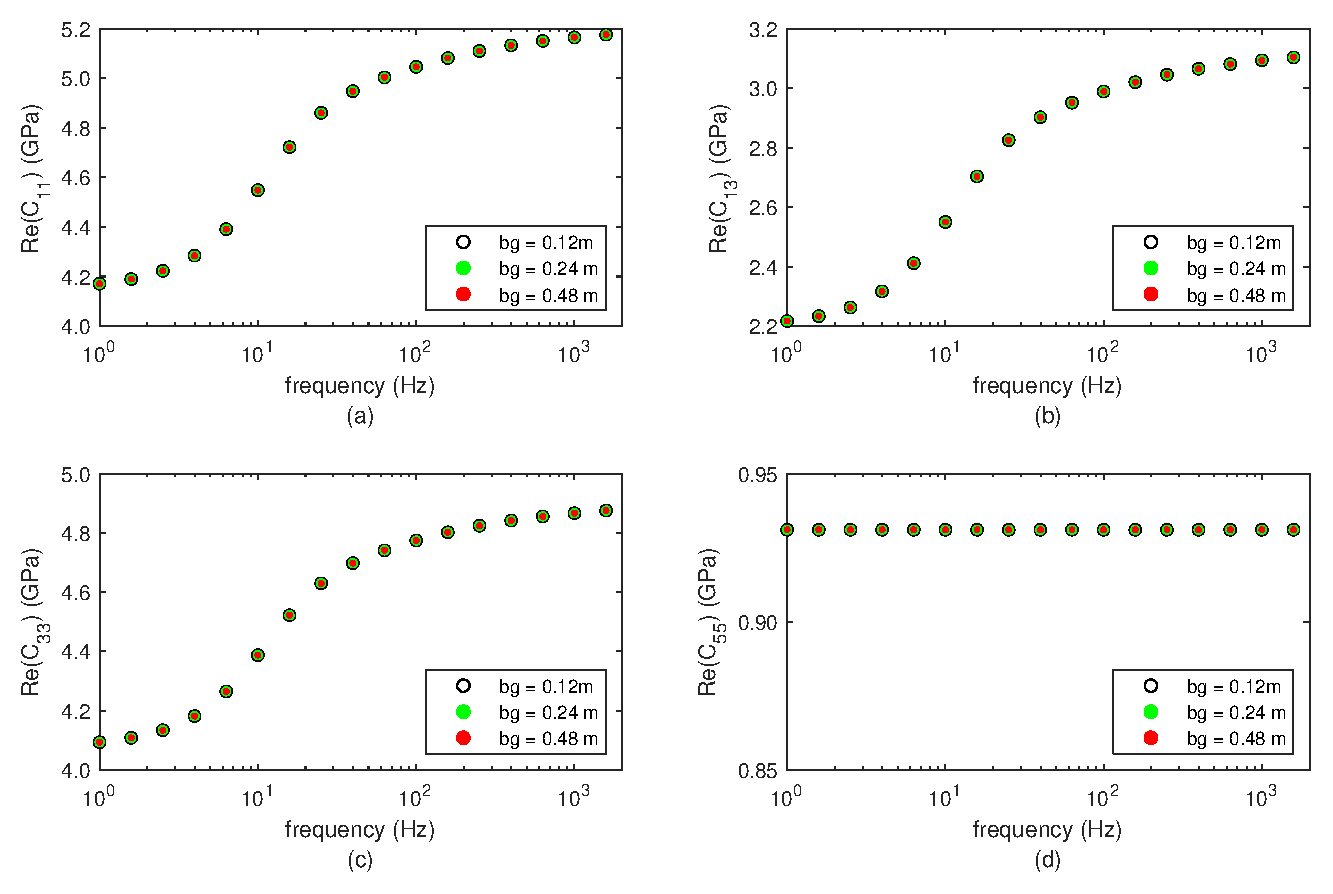
\includegraphics[width=110mm, height=80mm]{Figure2.eps}
\caption{Real part of the non-zero equivalent moduli as a function of frequency resulting from the homogenization of a thin layer composed of a sequence of two poroelastic sandstone beds, B1 and B2, embedded within  half-spaces $\Lambda_1$ and $\Lambda_2$ deemed impermeable for seismic frequencies (Tables \ref{table.1} and \ref{table.2}). The moduli are obtained using three different samples $\Omega_e$ (Figure \ref{fig.1}) that consider background thicknesses bg equal to 0.12 m, 0.24 m and 0.48 m, respectively.}
\label{fig.2}
\end{figure}

Figure \ref{fig.2} shows plots of the real part of the non-zero equivalent moduli as a function of frequency obtained using samples that consider background thicknesses equal to 0.12 m. 0.24 m and 0.48 m, respectively. The results demonstrate that the estimated moduli are independent of the thickness of the sampled background, which implies that the only influence the background has is to affect the BC at the respective thin layer boundaries. 
The homogenized medium is
characterized by vertical transverse isotropy (VTI), which results from the stratification   of the two sandstones that constitute the thin layer. Therefore, the elements $C_{15}$ and $C_{35}$ of its stiffness matrix are zero. Notice as well that $\Re(C_{55})$  (Figure \ref{fig.2}d) is not frequency-dependent. This is because the shear relaxation oscillatory test, which is the analogous to a normal-incident S-wave, generates shear strains and stresses components  parallel to the bedding planes of the thin layer. Consequently, such shear components cannot induce fluid pressure gradients for FPD to take place. Moreover, this element reads $C_{55} = \langle \sigma_{13}\rangle\,/(\,2\, \langle \varepsilon_{13} \rangle\,)$ and it can be shown that this is equivalent to $C_{55}  =\left( \sum_i f_i/\mu_i \right)^{-1}$, where $f_i$ is the height fraction of the $i$th layer and $\mu_i$ is the corresponding shear modulus \cite{Backus1962, Salamon1968}. This value is 0.93 GPa for our example. The moduli  $C_{11}$, $C_{13}$ and $C_{33}$ are affected by FPD effects and therefore present a frequency-dependent behavior. Specifically, the pressure gradient for FPD is controlled by the water-saturated region due to its lower compressibility compared to the CO$_2$-saturated counterpart. As a consequence, the deformation induced by the compressional relaxation oscillatory tests creates higher pressure in the water-saturated region that equilibrates when water diffuses into the CO$_2$-saturated pores of the adjacent sandstone bed. Similarly, the transition frequency of these moduli is controlled by the viscosity of water and thickness of the corresponding bed. Using Equations \eqref{Eq.3} and \eqref{Eq.5}, we find that this transition frequency is approximately 11.8 Hz. 

\begin{figure}[!ht]
\centering
        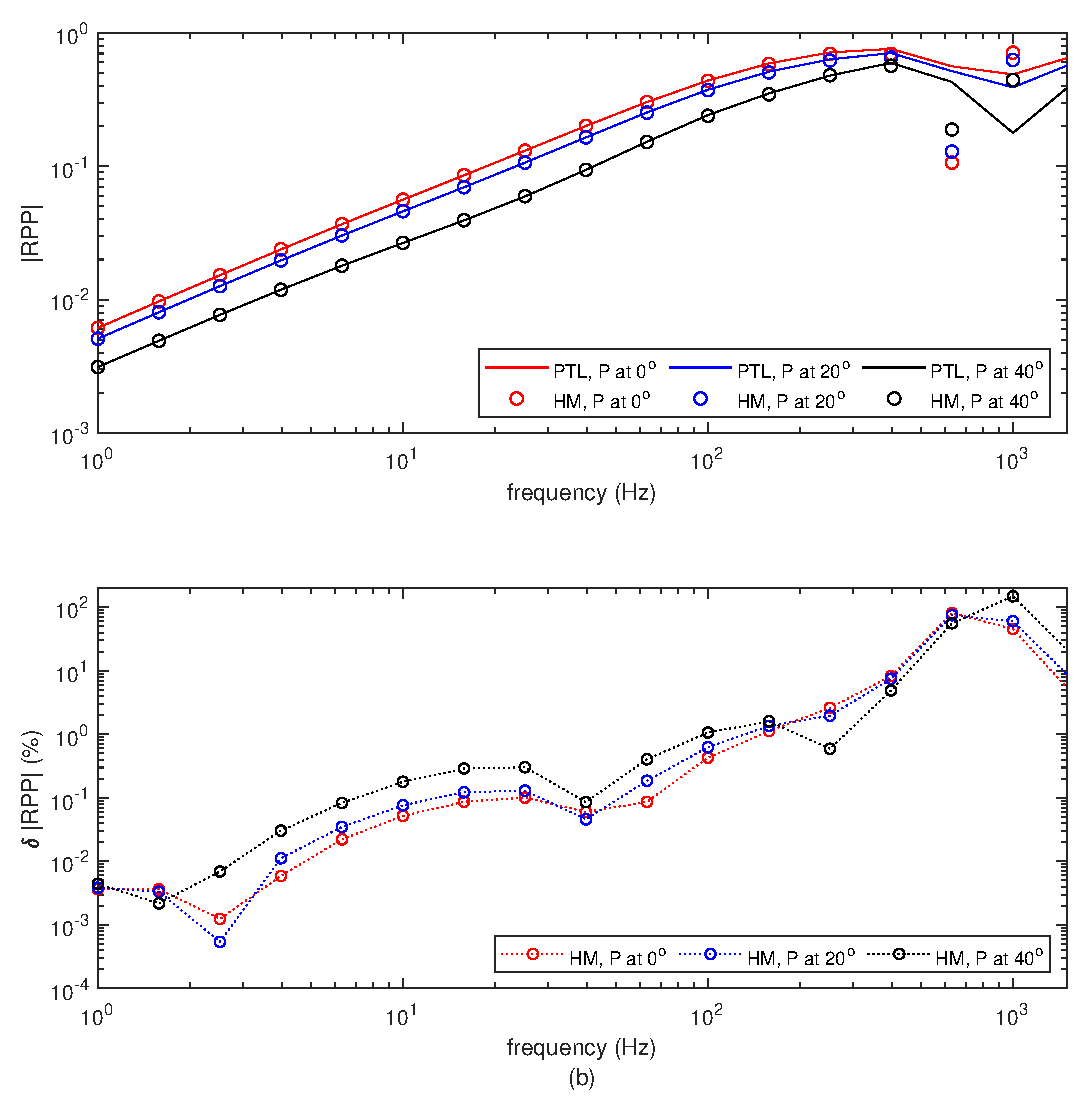
\includegraphics[width= 130mm, height=120mm]{Figure3.eps}
\caption{ (a) Absolute value of the PP reflection coefficients as a function of frequency for several angles of incidence calculated for the model consisting of the poroelastic thin layer comprised by two sandstone beds embedded in elastic half-spaces (curves labeled PTL) and for the analogous model where the thin layer is replaced by its homogenized viscoelastic equivalent (curves labeled HM). (b) Percentage errors of the absolute values of the PP reflection coefficients as a function of frequency calculated for the model using the homogenized medium.}
\label{fig.3}
\end{figure}

Next, we present the reflectivity results using the homogenized medium as well as a comparison against the results obtained using the poroelastic thin layer. 
Figure \ref{fig.3}a shows the absolute value of the PP reflection coefficients with respect to frequency for three different angles of incidence calculated for the poroelastic thin-layer model consisting of two sandstone beds that is embedded in elastic half-spaces and for the analogous model where the poroelastic thin layer is replaced by its homogenized viscoelastic equivalent. Notice that the reflectivities obtained using the homogenized medium show a good agreement with the reference reflectivities, which demonstrates that estimated moduli are capable to reproduce the reflectivity response of the porous thin layer. In more detail,
Figure \ref{fig.3}b shows the percentage errors of the absolute value of the PP reflection coefficients as a function of frequency of the model using the homogenized medium for the same angles of incidence used in Figure \ref{fig.3}a. 
Here, we remark that for the model using the homogenized medium, reverberations in the reflection coefficients are expected to appear at a frequency close to 325 Hz for normal incidence, as the first resonance occurs when the predominant wavelength is  equal to four times the thickness of the thin layer. Thus, for frequencies equal or higher than the resonance frequency, different behaviors in the reflectivities from both models are expected. For frequencies below 325 Hz, our results show that the PP reflection coefficients obtained using the homogenized medium reproduce, with errors below 3 \%, those obtained using the poroelastic thin model. 

%*****************
%Discussion
%*****************
\section{Discussion}
%We have proposed a method to homogenize porous thin layers with non-periodic heterogeneities. 
We have shown that considering a portion of the background in the sample 
permits to  naturally incorporate the BC at the interface between the background and the thin layer into the homogenization procedure. In the following, we investigate the impact that substituting the background by different BC has on the estimated moduli. To this end, we test samples that disregard the background and, instead, incorporate the following BC on their pertinent boundaries: fully periodic BC and  no-flow with periodic BC for displacements and tractions. Finally, we discuss about possible extensions of the proposed homogenization methodology to thin layers with more complex heterogeneous structures as well as  particular limitations of the method such as those associated with backgrounds that behave as permeable for the frequencies of interest.

\subsection{Testing samples that disregard the background}
%We substitute the presence of the background by different BC to test their effects on the estimated moduli. 
%To this end,
%we take samples $\Omega_p$ that consist only of a representative section of the poroelastic thin layer of the model described in the Results section.
%This is $\Omega_p = \Omega_e  \setminus \Omega_b $ (Figure \ref{fig.1}b). Then, we impose the fully periodic and the no-flow with periodic BC for displacements and tractions on the pertinent boundaries for each test, respectively. 

\subsubsection{Fully periodic BC}
\begin{figure}[!ht]
\centering
        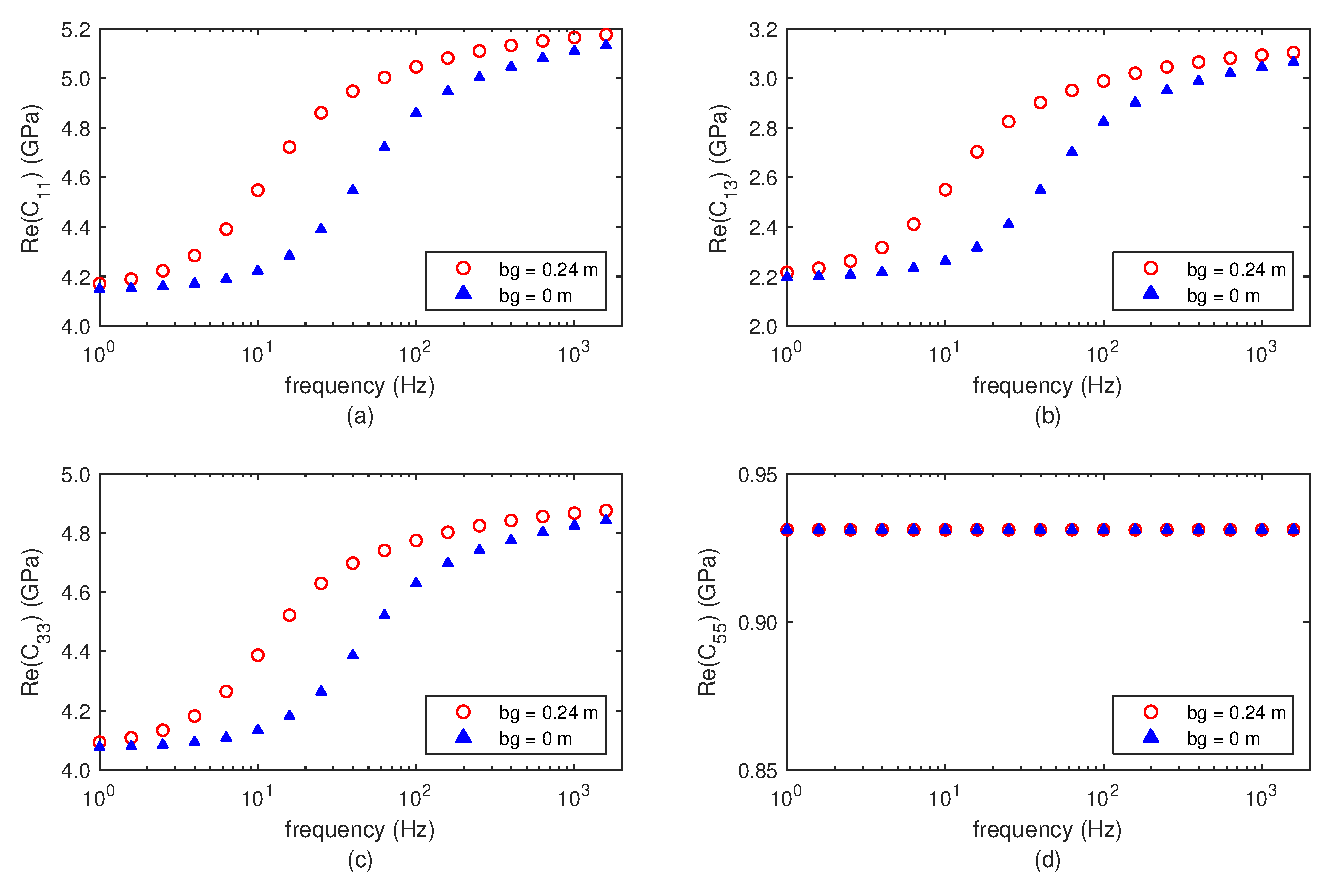
\includegraphics[width= 120mm, height=80mm]{Figure4.eps}
\caption{Real part of the non-zero equivalent moduli as a function of frequency obtained after homogenizing the poroelastic thin layer considered in the Results section using samples $\Omega_e$ and $\Omega_p$, respectively. Sample $\Omega_e$ considers a background thickness bg = 0.24 m, while sample $\Omega_p$ disregards it (bg = 0 m) and, instead, incorporates fully periodic BC on the pertinent boundaries. }
\label{fig.4}
\end{figure}

We take samples $\Omega_p$ that consist only of a representative section of the poroelastic thin layer of the model described in the Results section. This is $\Omega_p = \Omega_e  \setminus \Omega_b $ (Figure \ref{fig.1}b). We homogenize this sample using the procedure described in the Theory and Methods section, but, in this case, the corresponding equations are applied only  over $\Omega_p$ and on its boundaries, respectively. 
This homogenization procedure is equivalent to considering the sample $\Omega_p$ as periodic. Since the sample is composed of two porous beds, it represents White's model of periodically alternating beds \cite{White1975}. Considering a similar model, \citeA{Favino2020} verify the agreement of the homogenized P-wave modulus obtained using the closed form proposed by \citeA{White1975} and their numerical homogenization with periodic BC, which is the method we apply to homogenize this sample.

Figure \ref{fig.4} shows the real part of the non-zero equivalent moduli as a function of frequency obtained using the sample $\Omega_p$. For comparison, we have also included the previously estimated moduli obtained using the sample $\Omega_e$ that incorporates part of the background as detailed in the previous section. The results show  a visible difference between the two sets of curves corresponding to $\Re(C_{11})$, $\Re(C_{13})$ and $\Re(C_{33})$, with a maximum of around 0.4 GPa. These discrepancies evidence the impact of the different BC incorporated in the homogenization procedures. For the proposed method, the  background in the sample imposes both a no-flow condition due to its impermeable character for the frequencies considered as well as continuity of displacements and tractions at the pertinent boundaries of the thin layer section. In contrast, the  homogenization procedure that disregards the background in the sample imposes periodicity of these variables on analogous boundaries. 
As previously explained, $C_{55}$ is not frequency dependent because it is unaffected by the fluid effects and its closed form computation yields a value of 0.93 GPa, which, in this case, both homogenization procedures reproduce.

\subsubsection{No-flow and periodic BC for displacements and tractions} 
In the previous sub-subsection, we have stated that the background induces a no-flow condition at the interfaces with the thin poroelastic layer, which results from its impermeable character for the frequencies considered, as well as continuity of displacements and tractions. Here, we investigate the extent to which this no-flow condition influences the estimation of the equivalent moduli. To this end, we  take a sample $\Omega_p$ of the thin-layer model used in the Results section, which disregards the background. Then, to incorporate in the homogenization procedure the no-flow condition imposed by the background, we formulate the corresponding BC on the relevant boundaries of the sample $\Omega_p$ as part of the  oscillatory relaxation tests. To achieve this, we replace Equation \ref{Eq.11} by
\begin{linenomath*}
\begin{equation}\label{Eq.14}
\begin{split}
& \nabla p \cdot \bm{\hat n}  = 0 \quad \text{on}\quad \Gamma_3^+ \, \cup \, \Gamma_3^-,\\
& p\vert_{\Gamma_1^+}-p\vert_{\Gamma_1^-} =0, \\
& \left(\bm{\sigma}\cdot \bm{\hat n} \right)\, \vert_{\Gamma_k^+}-\left(\bm{\sigma}\cdot \bm{\hat n} \right)\, \vert_{\Gamma_k^-} = \bm{0},\\
&\left( \frac{\kappa}{\eta} \nabla p \cdot \bm{\hat n} \right) \, \vert_{\Gamma_1^+} -\left( \frac{\kappa}{\eta} \nabla p \cdot \bm{\hat n} \right) \, \vert_{\Gamma_1^-} = 0.
\end{split}
\end{equation}
\end{linenomath*}

The first line defines the no-flow condition at the top and bottom boundaries of the sample $\Omega_p$. All other steps of the homogenization procedure are the same as the ones specified by Equations \eqref{Eq.6} to \eqref{Eq.13}, but applied over $\Omega_p$ and on its boundaries.

\begin{figure}[!ht]
\centering
        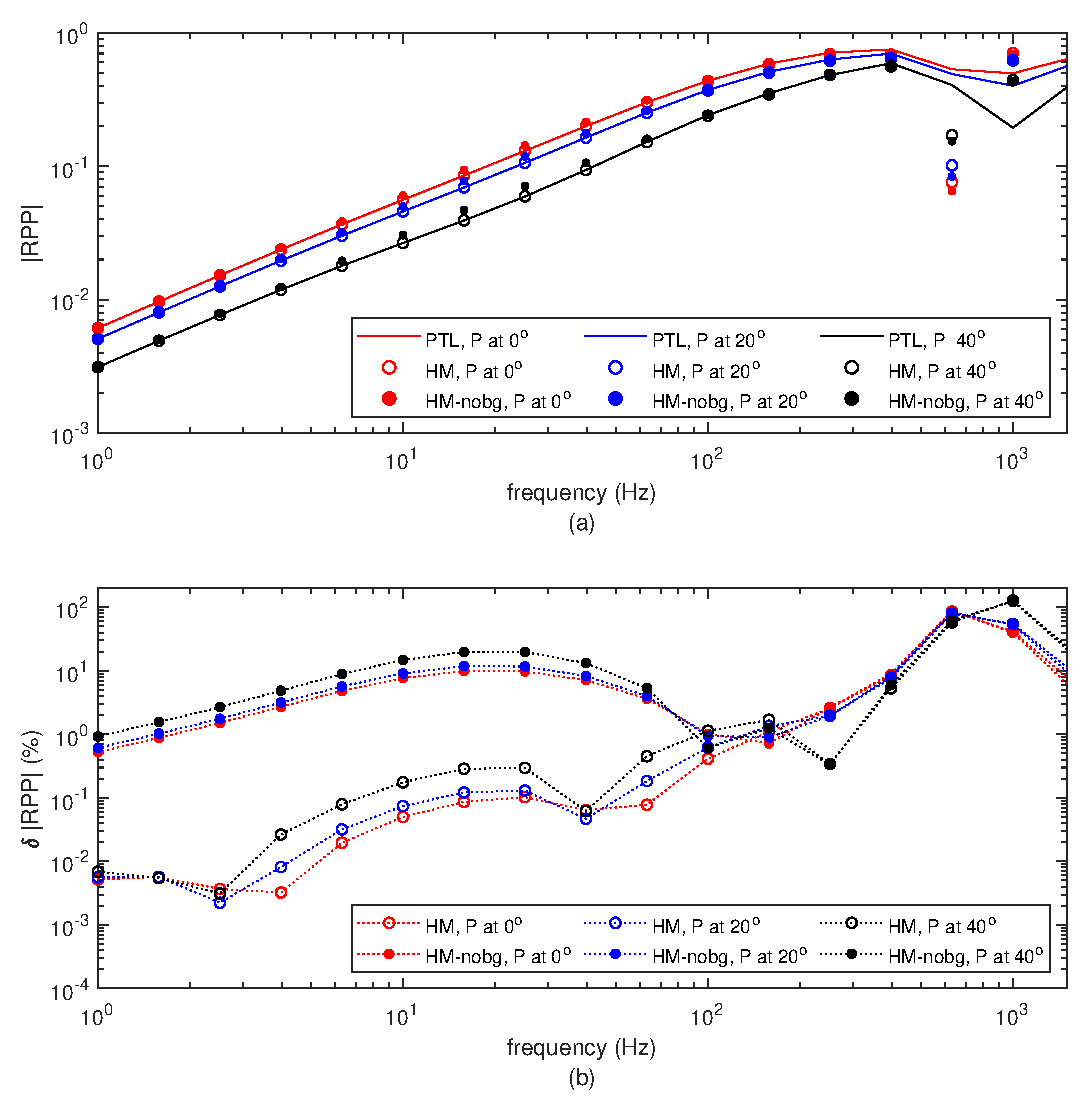
\includegraphics[width= 120mm, height=80mm]{Figure5.eps}
\caption{Real part of the non-zero equivalent moduli as a function of frequency obtained after homogenizing the thin-layer model considered in the Results section using samples $\Omega_e$ and  $\Omega_p$, respectively. Sample $\Omega_e$ considers a background thickness bg = 0.24 m, while sample $\Omega_p$ disregards it, and, instead, applies no-flow BC on the pertinent boundaries of the sample (nf, bg = 0 m) to emulate the impermeable character of the background.}
\label{fig.5}
\end{figure}

Figure \ref{fig.5} compares the real part of the non-zero equivalent moduli obtained with the homogenization procedure that applies the no-flow BC on the pertinent boundaries of a sample $\Omega_p$ against those obtained after applying the proposed method over a sample $\Omega_e$ that includes part of the embedding background. These results show that both procedures yield the same moduli. This further implies that, to homogenize a stratified porous thin layer comprised of a sequence of homogenous beds, it is sufficient to account for the no-flow condition induced by the background on the relevant boundaries of a sample $\Omega_p$. This outcome also suggests that, for this type of poroelastic thin layers, to impose either continuity of displacements and tractions at the the thin-layer-background interface on a sample $\Omega_e$ or periodicity of these quantities on analogous boundaries on a sample $\Omega_p$ do not have any impact on the estimation of the equivalent moduli.
This is likely to be a consequence of the uniform stress-strain distribution along the background-thin layer interfaces resulting from the homogeneous character of the beds. In the following, we therefore examine the effect that stress-strain concentrations at the background-thin layer interfaces has on the equivalent moduli.

Next, we consider a modified version of the thin-layer model used in the Results section, in which the upper bed B1 contains inclusions as shown in Figure \ref{fig.6}. We remark that the proposed homogenization procedure specifically addresses porous thin layers composed of homogeneous beds, mainly because this assumption facilitates the verification of the reflectivity response by semi-analytical means. However, the methodology, as we show in the current example, can be applied to porous thin layers presenting more complex heterogeneous structures. Nonetheless, a formal verification of the reflectivity response would still be required as we further discuss in the next subsection. Taking this into consideration, the following comparison of BC focuses on assessing the capability of the methods to reproduce, in a physically meaningful way, the actual stress and strain concentrations that the inclusions induce at the interface of the thin layer with the embedding background and therefore, their ability to incorporate those strain-stress concentrations in the estimation of the equivalent moduli.

As stated above, the new model shown in Figure \ref{fig.6} incorporates  inclined band-shape inclusions in the CO$_2$-saturated region, where the bands have one of their tips terminating at the upper boundary of the thin layer. These inclusions have stiffer mechanical properties and a lower permeability than the embedding sandstone: $K_m$ = 33.1 GPa,  $\mu$ = 29.2 GPa, $\kappa$ = $10^{-9}$ D, $K_s$ = 37 GPa, $\rho_s$ = 2700 g/kg$^3$ and $\phi$ = 0.05. The fluid properties correspond to those of water as specified in Table \ref{table.2}. We homogenize this poroelastic thin layer applying both the homogenization procedure that formulates the no-flow BC on the pertinent boundaries of a sample $\Omega_p$  and the proposed homogenization procedure that uses a sample $\Omega_e$. (Figure \ref{fig.6}).

\begin{figure}[!ht]
\centering
        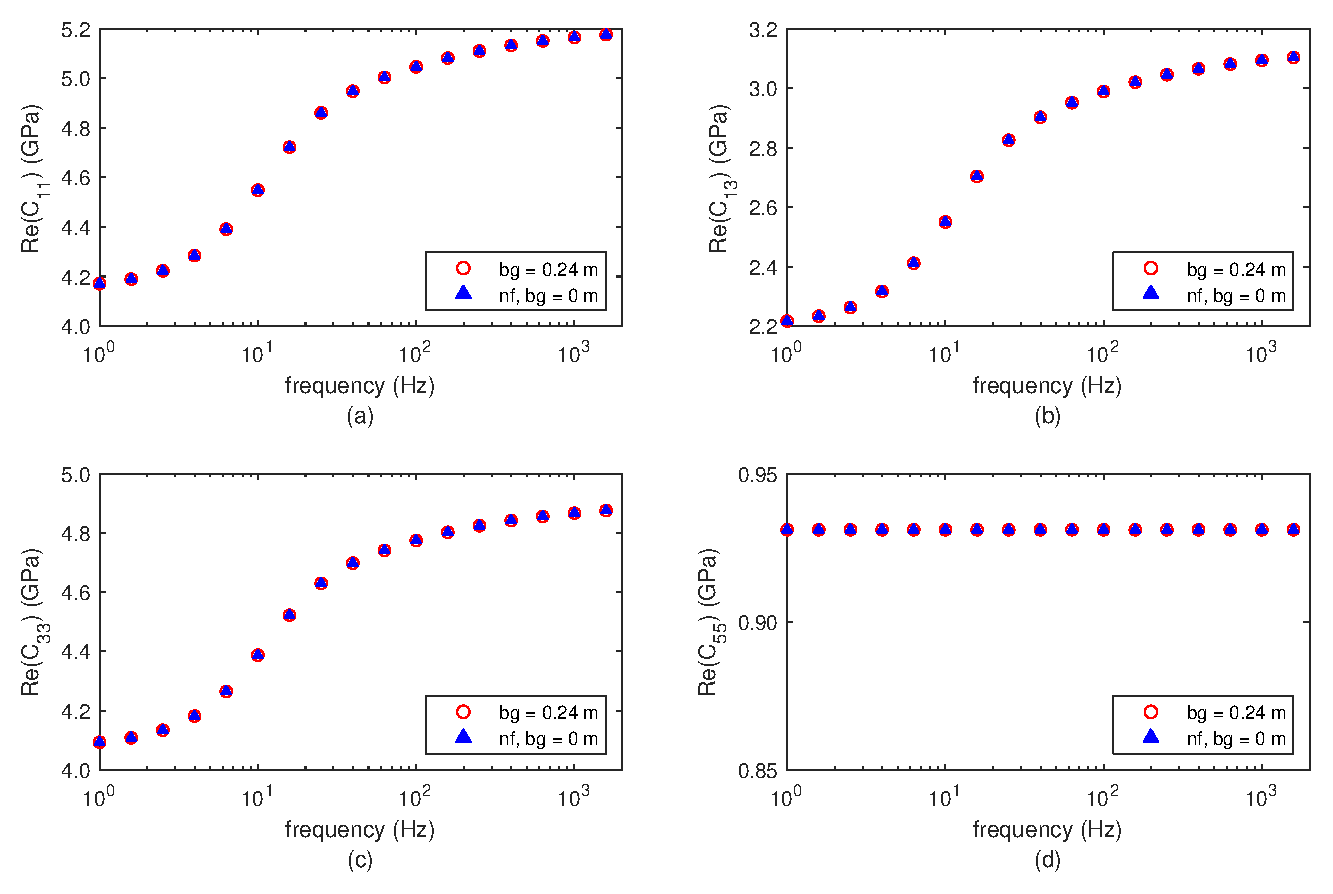
\includegraphics[width= 80mm, height=70mm]{Figure6.eps}
\caption{Poroelastic thin layer embedded in impermeable half-spaces $\Lambda_1$ and $\Lambda_2$. This model consists of the same sandstone beds B1 and B2 considered in the Results section. However, the upper sandstone contains inclined band-shape inclusions where the bands have one of their tips terminating at upper boundary of the thin layer. The light blue boxes represent the samples $\Omega_e$ and $\Omega_p$ used by the proposed homogenization and the one that imposes a no-flow BC on the relevant boundaries to emulate the impermeability of the background, respectively.}. 
\label{fig.6}
\end{figure}

\begin{figure}[!ht]
\centering
        \includegraphics[width= 120mm, height=80mm]{Figure7.eps}
\caption{Real part of the equivalent moduli as a function of frequency obtained after the homogenization of the poroelastic thin layer shown in Figure \ref{fig.7} using samples $\Omega_e$ and  $\Omega_p$, respectively. Sample $\Omega_e$ considers a background thickness bg = 0.24 m,while sample $\Omega_p$ disregards the it, and instead, imposes no-flow BC on the relevant boundaries of the sample (nf, bg = 0 m) to emulate the impermeable character of the background.}. 

\label{fig.7}
\end{figure}

\begin{figure}[!ht]
\centering
        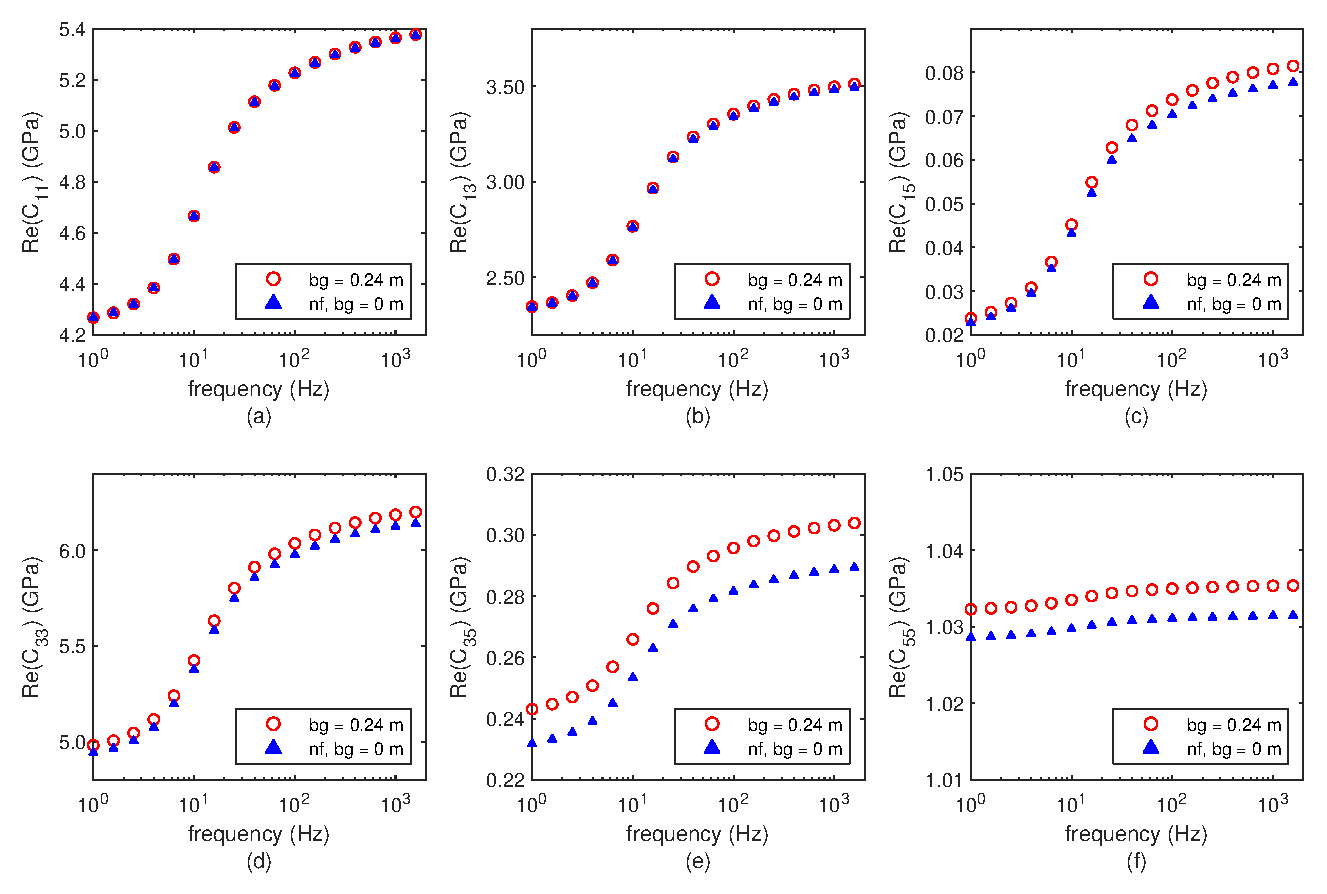
\includegraphics[width= 140mm, height=160mm]{Figure8.eps}
\caption{Maps of the real part of the vertical stress component obtained for the thin layer samples a) $\Omega_e$  and b) $\Omega_p$ (Figure \ref{fig.6}). Maps of the real part of the vertical strain component obtained for the same samples c) $\Omega_e$  and d) $\Omega_p$. 
The sample $\Omega_e$ considers a background thickness bg = 0.24 m.
The maps are obtained in response to applying the vertical compressional oscillatory test for a frequency of 25.1 HZ.}
\label{fig.8}
\end{figure}

Figure \ref{fig.7} shows the real part of the  equivalent moduli as a function of frequency obtained after applying the two aforementioned homogenization procedures.
The results show that there is some disagreement between the moduli estimations from the different methods.
This is likely to be related to differences in the regions affected by the stress-strain concentrations. To further investigate this aspect, we compare the corresponding stress and strain density maps obtained in response to the vertical compressional relaxation test for a frequency of 25.1 Hz. Figures \ref{fig.8}a and \ref{fig.8}b show maps of the real part of the vertical stress components for sample $\Omega_e$ that includes background with thickness bg = 0.24 m and for  sample $\Omega_p$, respectively. Similarly, Figures \ref{fig.8}c and \ref{fig.8}d show maps of the real part of the vertical strain components for the same samples  $\Omega_e$ and $\Omega_p$, respectively, for the same oscillatory test. Notice that, in both cases, the vertical compressional test creates stress-strain concentrations in the vicinity of the tips of the inclusions. However, the regions affected around the upper edges of the inclusions are different for the different samples. For the sample $\Omega_e$, these stress-strain concentrations affect a region in the background in the vicinity of the upper interface with the thin layer (Figures \ref{fig.8}a and \ref{fig.8}c). In contrast, for the sample $\Omega_p$  the corresponding stress-strain concentrations affect a region inside the thin layer in the vicinity of its bottom boundary as a consequence of the periodic character of the BC for displacements and tractions (Figures \ref{fig.8}b and \ref{fig.8}d), which is an artifact due to the inappropriate BC. This shows that the homogenization procedure that formulates the no-flow BC on the relevant boundaries of $\Omega_p$ considers an additional region of stress-strain concentration at the bottom boundary of the thin layer section when performing the averaging of these components. Hence, applying the proposed homogenization methodology is likely to reproduce more closely the actual stress-strain concentrations induced at the interface with the background. We also note that the induced stress-strain concentrations in the background imply that the considered background thickness should surpass this region to avoid the appearance of non-physical stress-strain concentrations at the bottom of the sample due to the periodic BC. For the reflectivity calculations, we can still assume that the upper half-space behaves as an homogeneous material despite of the region affected by the strain-stress concentrations because this region is in general much smaller than the considered wavelength. 

In this sub-subsection, we have shown that for the homogenization of stratified thin layers consisting of a sequence of homogeneous poroelastic beds embedded in impermeable background, it is sufficient to impose no-flow BC on the relevant boundaries of a sample that takes only a representative section of the thin layer. This is, however, no longer the case for poroelastic thin-layer models that exhibit more complex heterogeneities, which can create stress-strain concentrations at the thin layer boundaries. For these latter cases, our results suggest that the proposed homogenization methodology can reproduce more reasonably the expected regions of stress-strain concentrations.

\subsection{Possible extensions and limitations of the proposed method}

\subsubsection{Homogenization of porous thin layers with complex heterogeneous structures}
In this work, we have proposed an homogenization method to find the viscoelastic equivalent of non-periodically stratified porous thin layers embedded in impermeable background. We considered this simple porous thin-layer model to be able to compute its reflectivity response by a semi-analytical technique (Appendix A) to validate the homogenization procedure. However, the proposed methodology  can be extended to homogenize porous thin layers that are strongly heterogeneous as it has been suggested in the previous subsection. In this case, to be able to take a representative sample $\Omega_e$, the thin layer should contain heterogeneities which, in the horizontal direction, are either periodical or statistically stationary as, for instance, those depicted in the bed B1 of Figure \ref{fig.6}. Nonetheless, for such models further research incorporating numerical wave propagation is needed to verify whether the reflectivities of the viscoelatic equivalent are in agreement with those of the heterogeneous porous thin layer. 

\subsubsection{Effect of the background permeability}
For this study, we have assumed that the background embedding the poroelastic thin layer is impermeable for the frequencies of interest. This assumption permits to represent the background as an elastic medium for seismic applications and, at the same time, confine FPD effects within the poroelastic thin layer for such frequencies.
These features are particularly amenable for finding the corresponding viscoelastic equivalent capable of reproducing the reflectivity response of the poroelastic thin layer, as it has been shown in the current study. Conversely, if the background behaves as permeable for the frequencies of interest, it would allow hydraulic communication with the porous thin layer and, consequently, FPD regimes other than the unrelaxed one would prevail. This  would further imply that, for reflectivity computations, both the background and the thin layer should be treated as poroelastic media to account for the dissipated energy due to FPD.  In this case, a viscoelastic representation of the porous thin layer, as the one proposed in this study, can produce significant reflectivity deviations because it cannot incorporate  FPD interactions at the interfaces with the background. Conversely, we have shown that a background with a permeability in the nano ($10^{-9}$) Darcy range behaves as impermeable for seismic frequencies. Similarly, the work of \citeA{Barbosa2016} shows the same impermeable behavior for a background presenting a permeability in the micro ($10^{-6}$) Darcy range. Many background lithologies of interest, such as intact shale and crystalline rocks, exhibit permeabilities in the range of nano  to micro  Darcies  \cite<e.g.,>{Mitchell2012, Fisher2017, Wenning2018, Zhao2018}. This can be considered as impermeable for seismic frequencies and  hence permits to represent the considered background-porous-thin-layer system by elastic and viscoelastic media, respectively.


%*****************
%Conclusions
%*****************
\section{Conclusions}
We have proposed a homogenization approach that naturally incorporates the appropriate boundary conditions to estimate the equivalent moduli of stratified thin layers composed of a finite non-periodic sequence of homogeneous poroelastic beds embedded in an impermeable background.
This is accomplished by, first, taking a sample that incorporates both a portion of the background and a representative section of the poroelastic thin layer to apply relaxation oscillatory tests and, second, by performing the averaging of stress and strain components only over the thin layer section of interest.
Our results show that the proposed methodology yields equivalent moduli capable of closely reproducing the reflectivity of the original stratified thin layers. In contrast, the equivalent moduli obtained under the traditional assumption of periodicity yields inaccurate results. We  have also shown that the same moduli are reproduced when we use a sample that disregards the background but its influence is accounted by imposing a no-flow BC on the relevant boundaries of this sample. However, our study suggests that this is no longer the case for thin layers containing heterogeneities that induce stress-strain concentrations at the interfaces with the background, since disregarding the background in the sample produces regions of stress-strain concentration that do not reflect the physically expected ones. For such cases, our study implies that the proposed homogenization procedure yields more reasonable estimates of the equivalent moduli than replacing the background by no-flow BC on the pertinent boundaries of the sample. This outcome further indicates that the proposed homogenization method can be applied to strongly heterogeneous poroelastic thin layers, even though further work that incorporate numerical wave propagation is needed to verify the reflectiviy response of such heterogeneous models and their viscoelastic equivalents. Our study also suggests that to ensure the impermeable character
of the background for the frequencies of interest is vital to confine the FPD effects within the thin layer so that the background and the poroelastic thin layer can be represented as elastic and viscoelastic media, respectively, for reflectivity calculations. In general, it is expected that background rocks with permeabilities in the micro Darcy range and lower behave as impermeable at seismic frequencies.



%*****************
%Appendix
%*****************
\appendix
\section{PP reflectivity  at an elastic-poroelastic interface}

\subsection{Governing equations}
We consider a model in $\mathbb R^2$ consisting of 
$m$-poroelastic layers  $\Omega_{p1}$,  $\Omega_{p2}$,\dots, $\Omega_{pm}$ that are embedded in elastic half-spaces $\Lambda_1$ and $\Lambda_2$. Furthermore, we denote as $\Pi_1$  the interface between the upper half-space $\Lambda_1$ and the uppermost poroelastic layer $\Omega_{p1}$ and as $\Pi_{(m+1)}$ the interface between the lowermost poroelastic layer $\Omega_{pm}$ and the lower elastic half-space $\Lambda_2$. To compute the  reflection coefficients, we formulate the corresponding poroelastic and elastic wave equations in the space-frequency domain. To specify the poroelastic wave equation,  we let $\bm{u}^p =\bm{u}^p( \bm{x}, \omega)$ and $\bm{w} =\bm{w}( \bm{x}, \omega)$  be the solid displacement vector and the relative fluid displacement vector, respectively for any position $\bm{x} \in z$ with $z=\{\Omega_{p1},\dots,\Omega_{pm}\}$  and angular frequency $\omega \in I$, with $I =(0,W]$. Moreover, we let $\bm {\sigma}^p$, be the total stress which acts upon the poroelastic medium. Then, we express the corresponding equation of motion as
\begin{linenomath*}
\begin{equation}\label{Eq.a1}
\begin{split}
& -\,\omega^2  \, \rho_b  \, \bm{u}^p -  \,\omega^2 \, \rho_f \, \bm{w}= \nabla . \, \bm{\sigma}^p \quad  \textrm{in} \quad z \times I, \\
& -\,\omega^2  \, \rho_f \, \bm{u}^p - \omega^2 g(\omega) \, \, \bm{w} + i \, \omega \, b(\omega) \, \bm{w} = - \nabla \, p_f \quad  \textrm{in} \quad z \times I.
\end{split}
\end{equation}
\end{linenomath*}
The constitutive equations are
\begin{linenomath*}
\begin{equation}\label{Eq.a2}
\begin{split}
& \bm{\sigma}^p = \mu \,  \left( \nabla \,\bm{u}^p + ({\nabla  \bm{u}^p})^T  \right) +  \left( \lambda \, \nabla . \, \bm{u}^p\, + \alpha \,M \, \nabla . \, \bm{w} \right) \bm{I}, \\
&p_f=- \alpha \, M \, \nabla . \, \bm{u}^p - M \, \nabla . \, \bm{w},  \end{split}
\end{equation}
\end{linenomath*}
where $\rho_b$ and $\rho_f$ are the bulk density of the saturated porous medium and the density of the pore fluid, respectively,  $\lambda$ is the undrained Lamé modulus, and $g(\omega)$ and $b(\omega)$ are the mass coupling and viscous coefficients, respectively. The required material properties are calculated as \cite<e.g.,>{Barbosa2016}
\begin{linenomath*}
\begin{equation}\label{Eq.a3}
\begin{split}
& \rho_b =(1-\phi)\rho_s + \phi \rho_f, \\
& \lambda= K_m - \frac{2}{3} \mu + \alpha^2 M, \\
& g(\omega) =  \frac{1}{\omega} \Im \left( \frac{\eta}{\kappa_d(\omega)} \right),\\
& b(\omega) = \Re\left( \frac{\eta}{\kappa_d(\omega)} \right),
\end{split}
\end{equation}
\end{linenomath*}
where $\rho_s$ is the density of the solid grain and $\kappa_d(\omega)$ is the dynamic permeability of the porous rock, which can be expressed as \cite{Johnson1987}
\begin{linenomath*}
\begin{equation}\label{Eq.a4}
    \kappa_d(\omega)=\kappa \left(\sqrt{1 + \frac{4 i \omega}{n_j \omega_B} }+ \frac{i \omega}{\omega_B}   \right) ^{-1}.
\end{equation}
\end{linenomath*}
Here, $\omega_B$ is  Biot's angular characteristic frequency $\omega_B = 2 \pi f_B$, with $f_B$ defined in equation \ref{Eq.1}, and $n_j$ is a pore geometry parameter. According to numerical and experimental studies \cite<e.g.,>{Charlaix1988, Sheng1988, Smeulders1992}, $n_j$ = 8 is a reasonable approximation for most porous media.

To formulate the elastic wave equation, we let $\bm{u}^e=\bm{u}^e (\bm{x},\omega)$ be the displacement vector for any position $\bm{x} \in n$ with $n = \{\Lambda_1,\Lambda_2\}$  and angular frequency $\omega \in I$, with $I =(0,W]$. We also let $\bm{\sigma}^e$ be the stress tensor field acting upon the medium. Then, we express the corresponding equation of motion as
\begin{linenomath*}
\begin{equation}\label{Eq.a5}
- \, \rho_b \,\omega^2 \, \bm{u}^e = \nabla . \, \bm{\sigma}^e  \quad  \textrm{in} \quad n \times I.
\end{equation}
\end{linenomath*}
The associated constitutive equation is given by
\begin{linenomath*}
\begin{equation}\label{Eq.a6}
\bm{\sigma}^e = \mu \,  \left( \nabla \, \bm{u}^e + ({\nabla  \bm{u}^e})^T  \right) + \lambda \,  \nabla . \, \bm{u}^e\,\, \bm{I}.
\end{equation}
\end{linenomath*}
 
\subsection{Solution for displacements}
We assume that a P-wave propagates downwards, with wavevector components in $\bm{\hat x_1}$ and  $\bm{\hat x_3}$, and strikes the interface $\Pi_1$.  Then, in the elastic half-spaces $n$, with $n =\{\Lambda_1,\Lambda_2\}$, the propagating modes  are P- and S-waves. In the poroelastic layers $z$, with $z=\{\Omega_{p1},\dots,\Omega_{pm}\}$, fast P-, slow P- and S-waves are present.

For a given poroelastic layer $z$, we write the total solid displacement $\bm{u}_z^p$  and relative fluid displacement $\bm{w}_z$ as
\begin{linenomath*}
\begin{equation}\label{Eq.a7}
\begin{split}
& \bm{u}_z^{p} =  \sum_r \bm{u}_{z\,r}^p, \\
& \bm{w}_z =  \sum_r \bm{w}_{z\,r},
\end{split}
\end{equation}
\end{linenomath*}
with $r=\{D_{P1},U_{P1},D_{P2},U_{P2},D_{S},U_{S}\}$. Here, $D$ and $U$ refer to the downgoing and upgoing waves, respectively, and subscripts $P1$, $P2$, and $S$ refer to fast P-, slow P- and S-waves, respectively,

For a given elastic-half space $n$,  we express the total displacement $\bm{u}_n^e$ as
\begin{linenomath*}
\begin{equation}\label{Eq.a8}
\bm{u}_n^{e} =  \sum_j \bm{u}_{n\,j}^e.
\end{equation}
\end{linenomath*}
Here, for $n =\Lambda_1 $,  $j=\{D_P,\,U_P,\,U_S\}$; otherwise, for $n =\Lambda_2 $, $j=\{D_P,\,D_S\}$. Subscripts $P$  and $S$ refer to P- and S-waves, respectively. 

We propose the solution for displacements in the form of scalar and vector potentials. Then, we express the displacements for the elastic half-spaces as
\begin{linenomath*}
\begin{equation}\label{Eq.a9}
\begin{aligned}
& \bm{u}_{n\,j_1}^e = \nabla \Phi^e_{n\,j_1},
\end{aligned}
\qquad
\begin{aligned}
& \bm{u}_{n\,j_2}^e = -  \nabla  \times \bm{\Psi}^e_{n\,j_2}.
\end{aligned}
\end{equation}
\end{linenomath*}
For $n =\Lambda_1 $,  $j_1 = \{U_P,\,D_P\}$,  while for $n =\Lambda_2 $, $j_1 = \{D_P\}$ and $j_2=j \setminus j_1$ for both cases. $\Phi^e_{n\,j_1}$ and $\bm{\Psi}^e_{n\,j_2}$ are the scalar potentials corresponding to solutions for P-waves and the vector potential corresponding to solutions for S-waves, respectively. The potentials can be specified as
\begin{linenomath*}
\begin{equation}\label{Eq.a10}
\begin{split}
&  \Phi^e_{n\,j_1} = E_{n\,j_1} \exp \left( i\, \bm{k}_{n\, j_1}\cdot \bm{x} \right), \\
& \bm{\Psi}^e_{n\,j_2} =  E_{n\,j_2} \exp \left( i\, \bm{k}_{n\, j_2} \cdot \bm{x} \right) \bm{\hat {x}_2}, 
\end{split}
\end{equation}
\end{linenomath*}
where $E_{n\,j_1}$ and $E_{n\,j_2}$ are the amplitudes for the scalar and vector potentials, respectively and $\bm{k}_{n \,j_1}$, and $\bm{k}_{n\, j_2}$ are the wavenumber vectors for the P- and S-waves, respectively. The wavenumber vectors can be expressed as $\bm{k}_{n j} = k_{nj} \, \bm{\hat {k}_{nj}}$, where $\bm{\hat {k}_{n\, j}}$ is the unit wavenumber vector and $k_{n\,j}$ is the scalar wavenumber for the corresponding wave $j$. This latter depends only on the properties of the medium and on the wave type, that is, P or S. The scalar wavenumber can be written as
\begin{linenomath*}
\begin{equation}\label{Eq.a11}
\begin{split}
& k_{n\,j_1}  = \omega \sqrt{\frac{\rho_n}{\lambda_n + 2 \mu_n}}, \\[10pt]
& k_{n\,j_2}  = \omega \sqrt{\frac{\rho_n}{ \mu_n}}.
\end{split}
\end{equation}
\end{linenomath*}
%write P and S wavenumber equation%

For the poroelastic layers, we also express the solid and relative fluid displacements in term of potentials
\begin{linenomath*}
\begin{equation}\label{Eq.a12}
\begin{aligned}
& \bm{u}_{z\,r_1}^p = \nabla \Phi^p_{z\,r_1},
\end{aligned}
\qquad
\begin{aligned}
& \bm{u}_{z\,r_2}^p = - \nabla \times \bm{\Psi}^p_{z\,r_2},
\end{aligned}
\end{equation}
\end{linenomath*}
%*************
\begin{linenomath*}
\begin{equation}\label{Eq.a13}
\begin{aligned}
& \bm{w}_{z\,r_1} = \nabla \Theta_{z\,r_1},
\end{aligned}
\qquad
\begin{aligned}
& \bm{w}_{z\,r_2} = -  \nabla \times \bm{T}_{z\,r_2},
\end{aligned}
\end{equation}
\end{linenomath*}
where  $r_1 = \{D_{P1},\,U_{P1},\,D_{P2},\,U_{P2}\}$ and $r_2=r\setminus r_1$, 
$\Phi^p_{z\,r_1}$ and $\Theta_{z\,r_1}$ are the scalar potentials corresponding to solutions for P1- and P2-waves for the solid and the relative fluid displacements, respectively. Likewise $\bm{\Psi}^p_{z\,r_2}$ and $ \bm{T}_{z\,r_2}$ are the vector potentials corresponding to solutions for S-waves for the solid and the relative fluid displacements, respectively. The scalar and vector potentials can be further specified as
\begin{linenomath*}
\begin{equation}\label{Eq.a14}
\begin{split}
&  \Phi^p_{z\,r_1} = B_{z\,r_1} \exp \left( i\, \bm{k}_{z\, r_1}\cdot \bm{x} \right), \\
& \Theta_{z\,r_1} =  W_{z\,r_1} \exp \left( i\, \bm{k}_{z\, r_1} \cdot \bm{x} \right), 
\end{split}
\end{equation}
\end{linenomath*}
\begin{linenomath*}
\begin{equation}\label{Eq.a15}
\begin{split}
& \bm{ \Psi}^p_{z\,r_2} = B_{z\,r_2} \exp \left( i\, \bm{k}_{z\, r_2}\cdot \bm{x} \right) \bm{\hat {x}_2}, \\
& \bm{T}_{z\,r_2} =  W_{z\,r_2} \exp \left( i\, \bm{k}_{z\, r_2} \cdot \bm{x} \right) \bm{\hat {x}_2}, 
\end{split}
\end{equation}
\end{linenomath*}
where $B_{z\,r1}$ and $W_{z\,r1}$ are the amplitudes of the scalar potentials corresponding to the solid and relative fluid displacements, respectively. Likewise, $B_{z\,r2}$ and $W_{z\,r2}$, are the amplitudes of the vector potentials corresponding to the solid and relative fluid displacements, respectively. Moreover, $\bm{k}_{z\, r_1}$ is the complex wavenumber vector for P1- and P2-waves and $\bm{k}_{z\, r_2}$ is the one for S-waves. Besides,  the  presence of the enclosing elastic half-spaces induces inhomogeneous waves in the poroelastic layers. This is because Snell's law imposes the continuity of the horizontal component of the wavenumber vectors across the different media and the presence of the an elastic media enforces this component to be real. Thus, attenuation can only prevail in the vertical direction. Then, we can specify the complex wavenumber vector as
\begin{linenomath*}
\begin{equation}\label{Eq.a16}
\bm{k}_{zr}= \bm{\varkappa}_{zr} - i\, \bm{\alpha}_{zr},
\end{equation}
\end{linenomath*}
where $\bm{\alpha}_{zr}$ is the attenuation vector which has only a component in $\bm{\hat{x}_3}$ and $\bm{\varkappa}_{zr}$ is the real wavenumber vector. This latter can be expressed as $\bm{\varkappa}_{zr} = \varkappa_{zr} \bm{\hat{\varkappa}}_{zr}$, where $\varkappa_{zr}$ and $\bm{\hat{\varkappa}}_{zr}$  are the  real wavenumber and unit vector, respectively. For a given incidence angle striking at the interface between the upper half-space and the top most poroelastic layer, Snell's law states that the horizontal component of the real wavevector of the traveling waves are equal to that of the incident wave $p_i$. This is $p_i = \bm{k}_{nj} \cdot \bm{\hat{x}_1} =\bm{\varkappa}_{zr} \cdot \bm{\hat{x}_1} = \varkappa_{zr} \sin(\theta_{zr})$, where $\theta_{zr}$ is the angle of the real wave vector with respect to the vertical. 
We express the missing vertical component of the complex wavenumber vector as follows: $\bm{k}_{zr} \cdot \bm{\hat{x}_3}= \varkappa_{zr}\cos (\theta_{zr}) - i\, \alpha_{zr}$, where $\alpha_{zr}$
is the attenuation factor. Following \citeA{Borcherdt1982} we find
\begin{linenomath*}
\begin{equation}\label{Eq.a17}
\begin{split}
& \varkappa_{zr}^2 =p_i^2 + \left(\Re\,[\left( k_{zr}^2 -  p_i^2\right)^{1/2}]\right)^2, \\
& \alpha_{zr}^2 = \left(\Im\,[\left( k_{zr}^2 -  p_i^2\right)^{1/2}]\right)^2, 
\end{split}
\end{equation}
\end{linenomath*}
where $k_{zr}$ is the complex wavenumber of the wave $r$, which depends on the wave type, that is P1, P2 or S, and the associated rock physical properties \cite{Borcherdt1973, Borcherdt1982}. To calculate the corresponding values, we follow the procedure employed by \citeA{Barbosa2016}.

\subsection{PP reflection coefficients}
If we assume that the amplitude of the incident P-wave is one, then the reflection coefficient $R_{PP}$ at the upper half-space is equal to $E_{\Lambda_1\, UP}$ (equation \eqref{Eq.a10}). To solve for the unknown amplitudes, we assemble a set of equations by imposing suitable continuity conditions at the interfaces.
In this regard, we distinguish two types of interfaces: elastic-poroelastic and purely poroelastic ones. At the elastic-poroelastic interfaces $\Pi_q$, with  $q=1$ and $q=m+1$, where $m$ is the number of poroelastic layers,
we impose continuity of solid displacements and tractions and we set to zero the relative fluid displacements \cite{Deresiewicz1963}
\begin{linenomath*}
\begin{equation}\label{Eq. a18}
\begin{split}
&  \left. \left(  \bm{u}_n^e -  \bm{u}_z^p \right) \right \rvert_{\Pi_q} = \bm{0} \,, \\
&  \left. \left(  \bm{t}_n^e -  \bm{t}_z^p \right) \right \rvert_{\Pi_q} = \bm{0} \,,\\
& \left.  \bm{w}_z \right \rvert_{\Pi_q} = \bm{0} \,.
\end{split}
\end{equation}
\end{linenomath*}
For $q=1$, the corresponding media are $n=\Lambda_1$ and $z=\Omega_{p1}$; for $q=m+1$, they are $n=\Lambda_2$ and $z=\Omega_{pm}$. Moreover, $ \bm{t}_n^e$ and $\bm{t}_z^p$ are the tractions on the $\Pi_q$ interface at the elastic and poroelastic sides, respectively. These tractions are $ \bm{t}_n^e =\bm{ \sigma}_n^e \cdot \bm{\hat{x}_3}$ and $ \bm{t}_z^p = \bm{\sigma}_z^p \cdot \bm{\hat{x}_3}$, respectively.

At the purely poroelastic interfaces $\Pi_q$ with $q=2,\dots,m$, we impose the continuity of solid displacements, relative fluid displacements, tractions, and fluid pressures \cite{Deresiewicz1963}
\begin{linenomath*}
\begin{equation}\label{Eq.19}
\begin{split}
&  \left. \left( \bm{u}_z^p -  \bm{u}_{(z+1)}^p \right) \right \rvert_{\Pi_q} = \bm{0} \,, \\
&  \left. \left(  \bm{w}_z -  \bm{w}_{(z+1)} \right) \right \rvert_{\Pi_q} = \bm{0} \,, \\
& \left . \left(  \bm{t}_z^p  - \bm{t}_{(z+1)}^p \right) \right \rvert_{\Pi_q}= \bm{0} \,,\\
&  \left. \left(  p_{f\,z} -  p_{f\, (z+1)} \right) \right \rvert_{\Pi_q} = 0 \,,
\end{split}
\end{equation}
\end{linenomath*}
where $z$ = $\Omega_{p(q-1)}$ and ($z+1$) = $\Omega_{pq}$. 
%Review the following ...
To complete the system of equations, we express the amplitudes of the relative fluid displacement in terms of the solid displacement through
 $\gamma_{zr}=W_{zr}/B_{zr}$. This ratio can be  obtained from the properties of the porous medium \cite{Barbosa2016}.


\section{PP reflectivity at an elastic-viscoelastic interface}
\subsection{Governing equations}
We assume a  domain in $\mathbb R^2$ consisting of an anisotropic viscoelastic layer $\Omega_v$  
embedded in the same elastic half-spaces $\Lambda_1$ and $\Lambda_2$ as in Appendix A. We denote as $\Pi_1$ the interface between the viscoelastic layer $\Omega_v$ and the upper half-space $\Lambda_1$ and as $\Pi_2$ the interface between the viscoelastic layer $\Omega_v$ and the lower half-space $\Lambda_2$.
 
To compute the reflection coefficients, we formulate the corresponding viscoelastic and elastic wave equations in the space-frequency domain. To specify the viscoelastic wave equation,  we let $\bm{u}^v =\bm{u}^v( \bm{x}, \omega)$  be the solid displacement vector for any position $\bm{x} \in \Omega_v$  and angular frequency $\omega \in I$, with $I =(0,W]$. Moreover, we let $\bm {\sigma}^v$, be the stress which acts upon the viscoelastic medium. Then, we express the corresponding equation of motion as
\begin{linenomath*}
\begin{equation}\label{Eq.b1}
- \, \rho_b^v \,\omega^2 \, \bm{u}^v = \nabla  \cdot \bm{\sigma}^v \quad  \textrm{in} \quad \Omega_v \times I, 
\end{equation}
\end{linenomath*}
where $\rho_b^v$ is the bulk density of the viscoelastic medium. Using Voigt's notation, the associated constitutive equation can be written as
\begin{linenomath*}
\begin{equation}\label{Eq.b2}
\setlength{\jot}{10pt}
\begin{split}
 &
 \begin{pmatrix}
 \sigma_{11}^v\\
 \sigma_{33}^v \\
  \sigma_{13}^v\\
 \end{pmatrix}
 =
   \begin{pmatrix}
  {C}_{11} & {C}_{13} & {C}_{15} \\
  {C}_{13} & {C}_{33} & {C}_{35} \\
  {C}_{15} & {C}_{35} & {C}_{55}\\
 \end{pmatrix}
  \begin{pmatrix}
  \varepsilon_{11}^v \\
  \varepsilon_{33}^v  \\
 2\,  \varepsilon_{13}^v \\
 \end{pmatrix},\\
 & \text{with} \qquad \varepsilon_{ij}^v =\frac{1}{2} \left(u_{i,j}^v + u_{j,i}^v\right).
 \end{split}
\end{equation}
\end{linenomath*}

The equations for the elastic wave and its constitutive relation are those presented in equations \eqref{Eq.a5} and \eqref{Eq.a6}.

\subsection{Solution for displacements}
We assume that an incident P-wave propagates downwards, with wavevector components in $\bm{\hat x_1}$ and  $\bm{\hat x_3}$, and strikes the interface $\Pi_1$. Then, the propagating modes present in the elastic media $\Lambda_1$ and $\Lambda_2$ are P- and S-waves. In the viscoelastic medium $\Omega_v$ quasi-P (qP)  and quasi-S (qS) body waves are present. 
Then, to find the total displacements in each medium, we sum the displacements produced by the corresponding propagating waves.

For the viscoelastic medium $\Omega_v$, the total displacement $\bm{u}^v$ is
\begin{linenomath*}
\begin{equation}\label{Eq.b3}
\bm{u}^v=  \sum_r \bm{u}_{r}^v.
\end{equation}
\end{linenomath*}
Here, $r=\{D_{qP},\,U_{qP},\, D_{qS},\,U_{qS}\}$, where subscripts $qP$ and $qS$ refer to $qP$- and $qS$-waves.
For the elastic half-spaces, the corresponding total displacements have been already detailed in equation \eqref{Eq.a8}.

We propose plane-wave solutions for the displacements. For the elastic media they take the following form
\begin{linenomath*}
\begin{equation}\label{Eq.b4}
\bm{u}_{nj}^e = E_{nj}\, \exp (- i \,\bm{k}_{nj} \cdot \bm {x} ) \; \bm{\hat {u}}_{nj},
\end{equation}
\end{linenomath*}

where, $n=\{ \Lambda_1,\Lambda_2 \}$. Furthermore, for $n =\Lambda_1 $,  $j=\{D_P,\,U_P,\,U_S\}$; otherwise for $n =\Lambda_2 $, $j=\{D_P,\,D_S\}$. $ E_{nj}$ is the amplitude of the plane wave,  $\bm{k}_{nj}$ is the 
wavenumber vector and its definition is the same as detailed in equations \eqref{Eq.a10} and \eqref{Eq.a11},
$\bm {x}$ is the position vector and $\bm{\hat {u}}_{nj}$ is the wave polarization unit vector that describes the direction of particle displacement. For P-waves, this vector is parallel to the wavenumber vector $\bm{k}_{nj}$ and for S-waves, this vector is perpendicular to it.

For the viscoelastic medium $\Omega_v$, the plane-wave solution takes the form
\begin{linenomath*}
\begin{equation}\label{Eq.b5}
\bm{u}_r^v = V_r\, \exp (- i \,\bm{k}_r \cdot \bm {x} ) \; \bm{\hat {u}}_r, 
\end{equation}
\end{linenomath*}
where $V_r$ is the amplitude of the plane wave, $\bm{k}_r$ is the complex wavenumber vector and $\bm{\hat {u}}_r$ is the wave polarization unit vector. In viscoelastic media, plane waves are in general inhomogeneous,
meaning that the real wavenumber vector $\bm{\varkappa}_r $  is not parallel to the attenuation vector $\bm{\alpha}_r$.  In a smilar way to equation \eqref{Eq.a16}, the complex wavenumber vector can be expressed as
\begin{linenomath*}
\begin{equation}\label{Eq.b6}
\bm{k}_r= \bm{\varkappa}_r - i\, \bm{\alpha}_r.
\end{equation}
\end{linenomath*}
We can also express the real wavenumber vector as $\bm{\varkappa}_r = {\varkappa}_r \, \bm{\hat{\varkappa}}_r $, where $\bm{\hat{\varkappa}}_r$ and ${\varkappa}_r$ are the real unit vector and  wavenumber, respectively. This latter can be related to the $r$-wave velocity $v_r$ as follows: ${\varkappa}_m = \omega/v_r$. For the present model, the presence of elastic half-spaces together with Snell's law implies that the horizontal component of the wavenumber vector is real. As a consequence, the attenuation vector $\bm{\alpha}_r$ has only a vertical component. Then, for a given incidence angle at the interface between the upper elastic half-space and the viscoelastic medium, Snell's law stipulates that the horizontal component of the wavevectors of the subsequent of the propagating waves are equal to that of the incident wave $p_i$, that is, $p_i = \bm{\varkappa}_{r} \cdot \bm{\hat{x}_1} = \bm{k}_{nj} \cdot \bm{\hat{x}_1}$.

The missing vertical component  $k_3=\bm{k}_r\cdot \bm{\hat{x}_3}$ of the wavevector $\bm{k}_r$ and the corresponding polarization vector $\bm{\hat{u}}$ of waves propagating in the viscoelastic medium can be found by solving the equation that arises after substituting equations \eqref{Eq.b2} and \eqref{Eq.b5} into \eqref{Eq.b1}. Here, without loss of generality, we assume that the amplitude $V_r$ is equal to 1. We also drop the subscript $r$. Then, the equation to solve is
\begin{linenomath*}
\begin{equation}\label{Eq.b7}
(\bm{\Gamma} - \rho_b^v \, \omega^2 \,\bm{I}) \,\bm{\hat{u}} = \bm{0},
\end{equation}
\end{linenomath*}
where
\begin{linenomath*}
\begin{equation}\label{Eq.b8}
\begin{split}
&\bm{\Gamma}=\bm{L}\,\bm{C}\,\bm{L}^T, \qquad  \text{with}  \\
&\bm{L}=\begin{pmatrix}  p_i & 0 & k_3\\ 0 & k_3 & p_i \end{pmatrix},
\end{split}
\end{equation}
\end{linenomath*}
where $\bm{C}$ is the stifness matrix as given by equation \eqref{Eq.b2}. Equation \eqref{Eq.b7} have solutions if $\bm{\det}(\bm{\Gamma} - \rho_b \, \omega^2 \,\bm{I}) = 0 $. This leads to a fourth-order equation in $k_3$, with solutions corresponding to vertical components of upgoing and downgoing qP- and qS-waves. After this, the corresponding unit polarization vectors $\bm{\hat{u}}$ can be found from equation \eqref{Eq.b7}. However, in anisotropic viscoelastic media, the direction of the real wavenumber vector  does not necessarily coincide with the direction of the average energy-flux vector $\bm{S}$ or ray path. Then, to select unequivocally the solutions for upgoing and downgoing waves, the  direction of the average energy flux should be established for the corresponding wavenumber vectors. This average energy flux vector $\bm{S}$ is the real part of the complex energy-flux vector $\bm{P}$, that is, $\bm{S} = \Re\,(\bm{P})$ \cite{Carcione1993, Cerveny2006}. The components of $\bm{P}$  can be calculated as \cite{carcione2007wave}
\begin{linenomath*}
\begin{equation}\label{Eq.b9}
P_i = -\frac{1}{2} \omega \, C_{ijkl}\, k_l\,\hat{u}_k \,\hat{u}_i^*.
\end{equation}
\end{linenomath*}
Here, indices take values of 1 and 3, and $\left(\cdot\right)^*$ denotes complex conjugate.
Furthermore, $C_{ijkl}$ are the components of the stiffness tensor. The conversion of the indices of the sitffness tensor from tensorial to  Voigt notation is as follows: double indices  $ij$ or $kl$ with values $11$, $13$, $31$ and $33$ convert to a single indices $1$, $5$, $5$ and $3$, respectively. For instance, $C_{3113}$ in tensorial notation is equivalent to $C_{55}$ in Voigt notation.

\subsection{PP Reflection coefficients}
As in in Appendix A, we assume that the amplitude of the incident P-wave is one and, hence, the reflection coefficient $R_{PP}$ at the upper half-space is then equal to $E_{\Lambda_1\, UP}$ (equation \eqref{Eq.b4}). To solve for the unknown amplitudes, we assemble a set of equations by imposing continuity of displacements and tractions at the elastic-viscoelastic interfaces $\Pi_q$ with $q=1,2$
\begin{linenomath*}
\begin{equation}\label{Eq.b10}
\begin{split}
&  \left. \left(  \bm{u}_n^e -  \bm{u}^v \right) \right \rvert_{\Pi_q} = \bm{0} \,, \\
&  \left. \left( \bm{t}_n^e  - \bm{t}^v  \right) \right \rvert_{\Pi_q} = \bm{0} \,.
\end{split}
\end{equation}
\end{linenomath*}
Here, $n$ = $\Lambda_q$, $\bm{t}_n^e$ and $\bm{t}^v$ are the tractions on the elastic and viscoelastic sides of the interface, respectively. Moreover, $\bm{t}^v =\bm{\sigma}^v \cdot \bm{\hat {x}_3} $. The traction $\bm{t}_n^e$ on the elastic side has already been defined in Appendix A.

\section*{Open Research}
The data used to create the figures containing the results of this study are available at the Zenodo repository via \url{https://doi.org/10.5281/zenodo.7692618} (doi:10.5281/zenodo.7692618) with Creative Commons Attribution 4.0 International Public License \cite{Sotelo2023}.

%%%%%%%%%%%%%%%%%%%%%%%%%%%%%%%%%%%%%%%%%%%%%%%%%%%%%%%%%%%%%%%%
%
%  ACKNOWLEDGMENTS
%%%%%%%%%%%%%%%%%%%%%%%%%%%%%%%%%%%%%%%%%%%%%%%%%%%%%%%%%%%%%%%%

\acknowledgments
This work is supported by the grant 200020-178946 from the Swiss National Science Foundation. J. G. R. gratefully acknowledges the financial support received from CONICET (PIP 11220210100346CO)
%% ------------------------------------------------------------------------ %%

%% References and Citations

%%%%%%%%%%%%%%%%%%%%%%%%%%%%%%%%%%%%%%%%%%%%%%%
%
% \bibliography{<name of your .bib file>} don't specify the file extension
%
% don't specify bibliographystyle
%%%%%%%%%%%%%%%%%%%%%%%%%%%%%%%%%%%%%%%%%%%%%%%

\bibliography{reference_SoteloEtal}

%%%%%
%\begin{thebibliography}{}


%\end{thebibliography}
%%%%%%


%Reference citation instructions and examples:
%
% Please use ONLY \cite and \citeA for reference citations.
% \cite for parenthetical references
% ...as shown in recent studies (Simpson et al., 2019)
% \citeA for in-text citations
% ...Simpson et al. (2019) have shown...
%
%
%...as shown by \citeA{jskilby}.
%...as shown by \citeA{lewin76}, \citeA{carson86}, \citeA{bartoldy02}, and \citeA{rinaldi03}.
%...has been shown \cite{jskilbye}.
%...has been shown \cite{lewin76,carson86,bartoldy02,rinaldi03}.
%... \cite <i.e.>[]{lewin76,carson86,bartoldy02,rinaldi03}.
%...has been shown by \cite <e.g.,>[and others]{lewin76}.
%
% apacite uses < > for prenotes and [ ] for postnotes
% DO NOT use other cite commands (e.g., \citet, \citep, \citeyear, \nocite, \citealp, etc.).
%
\end{document}




%




